\documentclass[a4paper, 12pt]{article}
\usepackage[T1]{fontenc}
\usepackage{lmodern}
\usepackage{color}
\usepackage{amsfonts}
\usepackage{epstopdf}
\usepackage{matlab}
\usepackage{booktabs}
%\documentclass{book}
\usepackage{blindtext}
\usepackage{hyperref}
\usepackage[brazil]{babel}
\usepackage{amssymb}
\usepackage[utf8]{inputenc}
\usepackage{amsmath}
\usepackage{indentfirst}
\usepackage{graphicx}
\usepackage{listings}
\usepackage{tcolorbox}
\usepackage{upgreek}
\usepackage{multicol,lipsum}
\usepackage[a4paper,
top=3cm, left=3cm, bottom=3cm, right=3cm]{geometry}
\usepackage{setspace}
\usepackage{multirow}
\usepackage{float}
\usepackage[dvipsnames]{xcolor}
\usepackage[table]{xcolor}
%\usepackage{pdflscape}
\usepackage[DIV=15]{typearea}
\usepackage[nottoc]{tocbibind}
\usepackage[sort,numbers]{natbib}
%\usepackage{cite}
\usepackage{matlab}

\usepackage[utf8]{inputenc}
\usepackage[T1]{fontenc}
\usepackage{lmodern}
\usepackage{graphicx}
\usepackage{color}
\usepackage{hyperref}
\usepackage{amsmath}
\usepackage{amsfonts}
\usepackage{epstopdf}
\usepackage[table]{xcolor}
\usepackage{matlab}

\lstdefinestyle{python}{
  language=Python,
  basicstyle=\ttfamily,
  keywordstyle=\color{blue},
  stringstyle=\color{orange},
  commentstyle=\color{gray},
  numbers=left,
  numberstyle=\tiny\color{gray},
  stepnumber=1,
  numbersep=5pt,
  backgroundcolor=\color{white},
  showspaces=false,
  showstringspaces=false,
  showtabs=false,
  frame=single,
  rulecolor=\color{black},
  tabsize=4,
  captionpos=b,
  breaklines=true,
  breakatwhitespace=false,
  title=\lstname,
  escapeinside={\%*}{*)},
  morekeywords={self},
  emph={MyClass,__init__},
  emphstyle=\color{red}
}


\documentclass[letterpaper]{article}
% bib pack %%%%%%%%%%%%%%%%%%%%%%%%%%%%%%%%%%%%%%%%%%%%%%%%%%%%%%%%%%%%%%%%%%%%%
\usepackage[utf8]{inputenc}
\usepackage{geometry}
    \geometry{left=3cm,right=2cm,top=2cm,bottom=2cm}
%
\usepackage[spanish]{babel}
%
\usepackage[fixlanguage]{babelbib}
    \bibliographystyle{babunsrt}
%
\usepackage{url}

\begin{document}
%\maketitle

\begin{titlepage}
	\begin{center}
		

\vspace{10pt}
%\begin{figure}[H][!ht]
%\centering
%
\includegraphics{puc-rio-logo.png}

%\end{figure}
\begin{figure}[!ht]
\centering

\includegraphics{images/puc-rio-logo.png}
\end{figure}
\huge{Análise de Séries Temporais}
        \vspace{70pt}
        
		\textbf{ENG1469}
		\textbf{\large{\\ }}
		
		\vspace{30pt}
		\textbf{\small{\\Lista Prática 04}}
		\vspace{75pt}
		
	\end{center}
	
	\begin{flushleft}
		\begin{tabbing}
		Aluno(a)\qquad\qquad\=\>Paloma Fernanda Loureiro Sette - 1621595\\
			Professor(a)\>Cristiano Fernandes\\
	\end{tabbing}
		  
	\end{flushleft}
	\begin{center}
		%\vspace{\fill}
		\vspace{215pt}
		Rio de Janeiro, 08 de Dezembro de 2024
	\end{center}
\end{titlepage}
%%%%%%%%%%%%%%%%%%%%%%%%%%%%%%%%%%%%%%%%%%%%%%%%%%%%%%%%%%%
\newpage
\tableofcontents
\thispagestyle{empty}

\newpage
\pagenumbering{arabic}

\newpage

%\newcommand{\listequationsname}{Lista de Equações}
%\newlistof{myequations}{equ}{\listequationsname}
%\newcommand{\myequations}[1]{%
%\addcontentsline{equ}{myequations}{\protect\numberline{\theequation}#1}\par}

%\listofmyequations
\newpage


\newpage

\listoffigures
\thispagestyle{empty}

\newpage
%%%%%%%%%%%%%%%%%%%%%%%%%%%%%%%%%%%%%%%%%%%%%%%%%%%%%%%%%
%%%%%%%%%%%%%%%%%%%%%%%%%%%%%%%%%%%%%%%%%%%%%%%%%%%

\newpage

\thispagestyle{empty}

\newpage

\section{Introdução}
A análise de séries temporais financeiras desempenha um papel fundamental na avaliação de risco e na modelagem de volatilidade nos mercados financeiros. Dentre as ferramentas mais utilizadas, destacam-se os modelos GARCH (Generalized Autoregressive Conditional Heteroskedasticity), que permitem capturar padrões de heterocedasticidade condicional presentes em séries de retornos financeiros, e o cálculo do Value at Risk (VaR), que quantifica o risco de perdas financeiras em um determinado horizonte temporal e nível de confiança.\\

Neste trabalho, empregamos dados históricos da ação da NVIDIA Corporation (NVDA) para investigar fatos estilizados associados aos retornos financeiros e construir modelos estatísticos para prever a volatilidade condicional e o VaR. A NVIDIA, sendo uma das empresas mais influentes no setor de tecnologia, oferece uma base rica para estudar as dinâmicas de mercado e os riscos associados à negociação de seus ativos.\\

Além disso, o trabalho segue uma abordagem prática e comparativa, avaliando diferentes especificações de modelos GARCH com distribuições normal e t-Student, utilizando métricas como AIC e BIC para seleção do modelo mais adequado. Por fim, aplicamos backtesting para validar os modelos propostos, garantindo que sejam robustos e confiáveis para a previsão de risco.

\newpage
\section{Objetivo}
O objetivo deste trabalho é modelar a volatilidade condicional dos retornos financeiros da ação da NVIDIA (NVDA) e calcular o Value at Risk (VaR) com base nos modelos GARCH. Especificamente, buscamos:

\begin{itemize}
    \item Identificar e analisar fatos estilizados dos retornos logarítmicos e aritméticos, como assimetria, curtose e autocorrelações.
    \item Ajustar e avaliar modelos $GARCH(p,q)$ com distribuições normal e t-Student, selecionando a configuração que melhor se adeque aos dados históricos da NVIDIA.
    \item Validar os modelos ajustados por meio de backtesting, verificando sua capacidade de prever riscos em diferentes níveis de confiança (1\% e 5\%).
    \item Estimar o VaR para $t+1$ e interpretar os resultados em cenários de aplicação prática, considerando a exposição financeira a ativos da NVIDIA.
\end{itemize}

Por meio dessas etapas, o trabalho oferece uma aplicação prática de métodos estatísticos e computacionais amplamente utilizados na gestão de riscos financeiros, conectando teoria e prática no contexto de séries temporais financeiras.




\newpage
\section{Preparando os dados}
A princípio, carregamos os dados necessários através da biblioteca \texttt{yfinance} do Python. Aqui, estamos extraindo os dados financeiros diários, em uma janela temporal de 8 (oito) anos. 


\begin{lstlisting}[style=python]
import yfinance as yf

# Baixando os dados financeiros da NVIDIA (NVDA) com a lib do yahoo finance
data = yf.download('NVDA', start='2016-12-03', end='2024-12-03')
# salvando em csv
data.to_csv('nvda_historical_data.csv')

\end{lstlisting} \\

Ao importarmos os dados, nos certificamos de que contém as informações necessárias, sobretudo a coluna de preços ajustados (\textit{\textbf{Adj Close}}).

\begin{figure}[H]
    \centering
    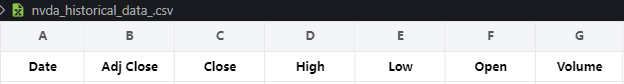
\includegraphics[width=0.8\textwidth]{images/dados_nvda.png}
    \caption{Colunas dos dados da série financeira de NVDA.}
\end{figure}

Por garantia, fizemos uma breve comparação com o que visualizamos na página indicada do Yahoo Finance e constatamos que os dados estavam em conformidade. É possível visualizar os dados através da URL: \url{https://finance.yahoo.com/quote/NVDA/history/}. 

\section{TAREFA 1: Fatos estilizados de séries de retornos financeiros}\label{sec:tarefa1}

\subsection{Parte I: Retornos Logarítmicos e Aritméticos}\label{subsec:tarefa1_pt1}

Nesta seção\footnote{O código Python utilizado para esta seção está disponível em \ref{apendice:codigo_tarefa1_pt1}.}, analisamos os retornos financeiros da ação da NVIDIA (NVDA), considerando tanto retornos logarítmicos quanto aritméticos. Para isso, os dados históricos de preços ajustados foram utilizados com o objetivo de capturar os movimentos reais de mercado.


\subsubsection{Cálculo dos Retornos}
Os retornos logarítmicos (\textit{Log Returns}) e aritméticos (\textit{Arithmetic Returns}) foram calculados utilizando as fórmulas:

\begin{equation}
r_{\text{log}} = \ln \left( \frac{P_t}{P_{t-1}} \right) \cdot 100
\end{equation}

\begin{equation}
r_{\text{arith}} = \left( \frac{P_t - P_{t-1}}{P_{t-1}} \right) \cdot 100
\end{equation}

onde $P_t$ é o preço de fechamento ajustado da ação no dia $t$, e $P_{t-1}$ é o preço de fechamento ajustado no dia anterior.

\subsubsection{Visualização Gráfica}
Os gráficos a seguir ilustram os retornos logarítmicos, aritméticos e a diferença entre eles ao longo do período analisado:

\begin{itemize}
    \item \textbf{Gráfico 1: Retornos Logarítmicos.} Este gráfico evidencia a volatilidade ao longo do tempo. Picos significativos podem ser observados em eventos de mercado importantes.
    \item \textbf{Gráfico 2: Retornos Aritméticos.} Similar aos logarítmicos, apresenta uma volatilidade alinhada, mas ligeiramente mais sensível a grandes variações de preço.
    \item \textbf{Gráfico 3: Diferença entre Retornos Aritméticos e Logarítmicos.} Apesar de geralmente pequenas, as diferenças tornam-se significativas em períodos de alta volatilidade, como durante o \textit{boom} das criptomoedas e outros eventos específicos.
\end{itemize}

\begin{figure}[H]
    \centering
    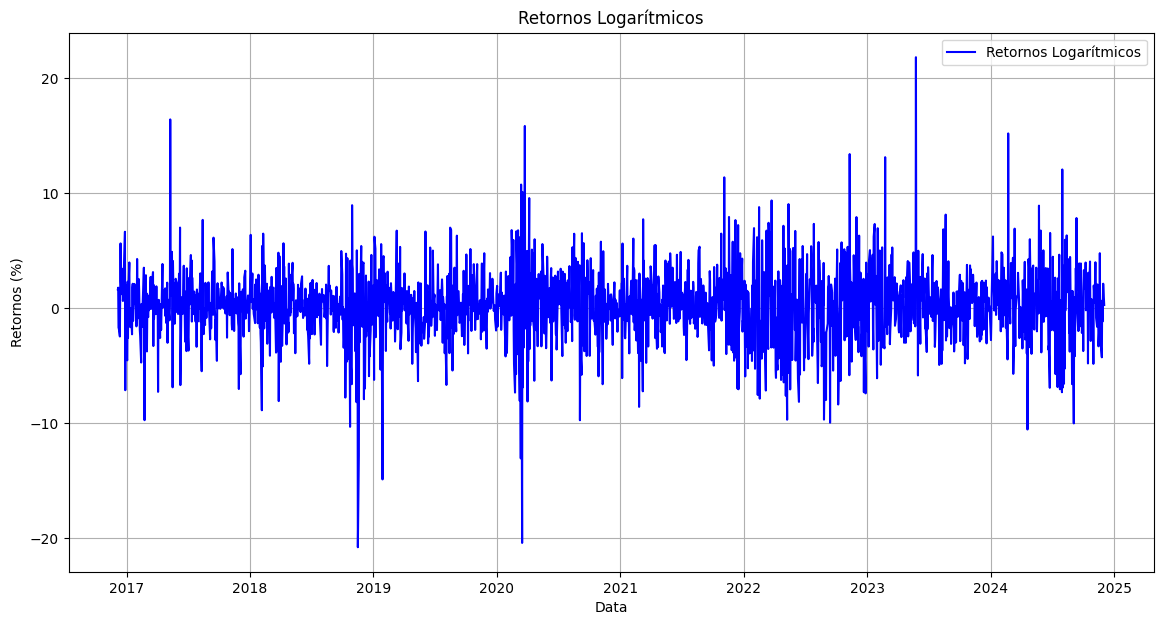
\includegraphics[width=0.8\textwidth]{images/log-retorno_TAREFA1.png}
    \caption{Retornos Logarítmicos da NVIDIA (NVDA).}
\end{figure}

\begin{figure}[H]
    \centering
    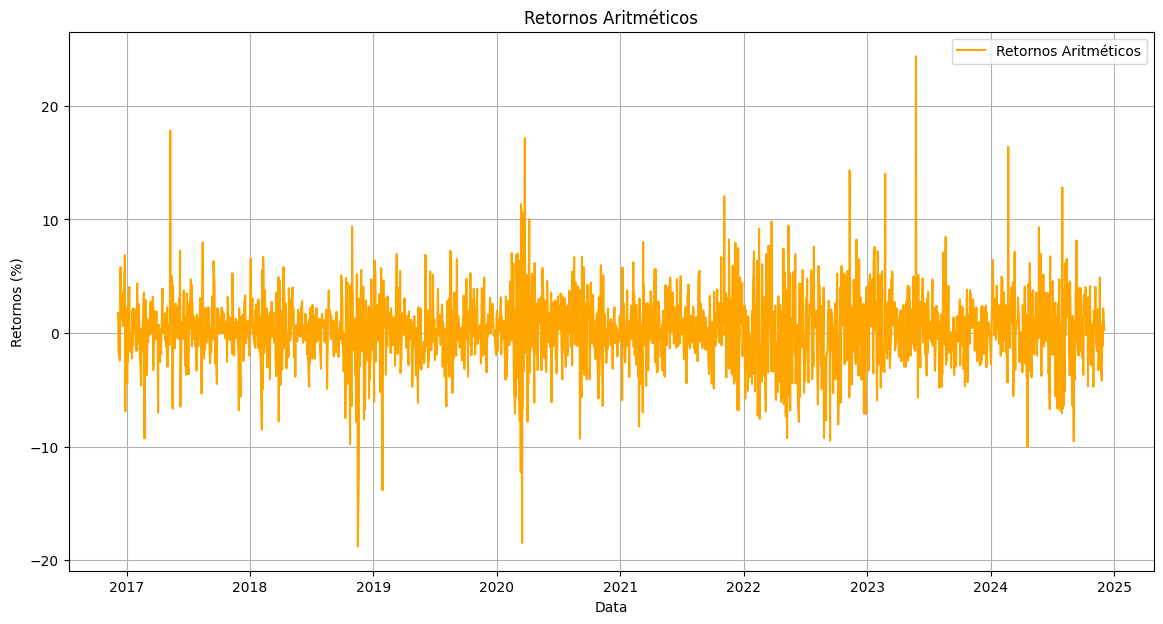
\includegraphics[width=0.8\textwidth]{images/arit-return_TAREFA1.png}
    \caption{Retornos Aritméticos da NVIDIA (NVDA).}
\end{figure}

\begin{figure}[H]
    \centering
    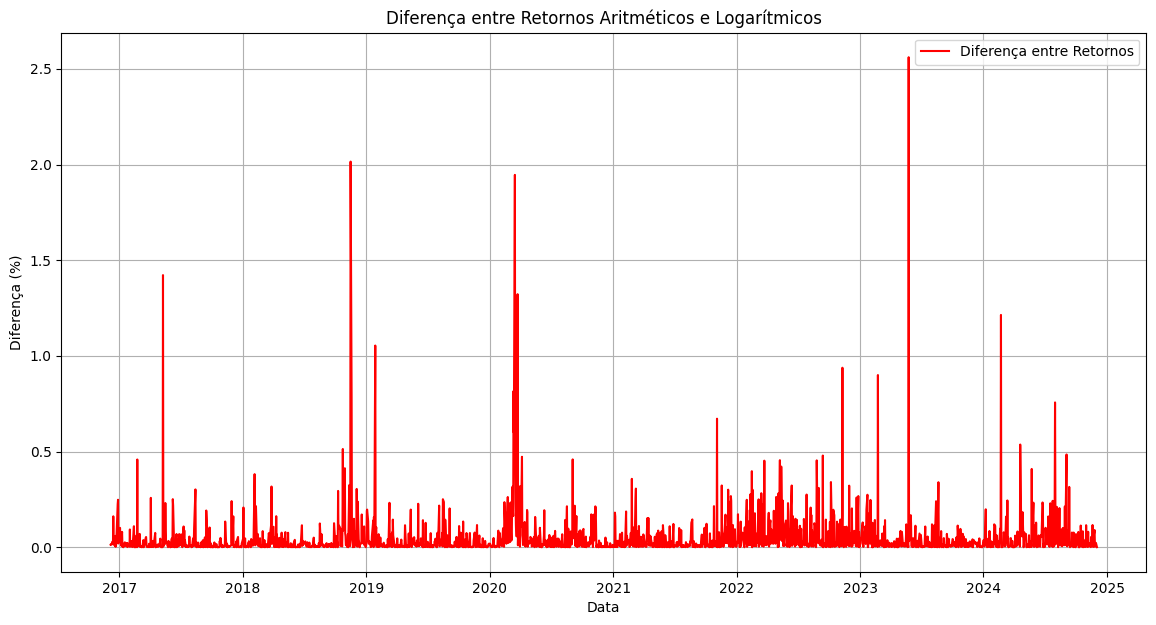
\includegraphics[width=0.8\textwidth]{images/diferencas_TAREFA1.png}
    \caption{Diferença entre Retornos Aritméticos e Logarítmicos da NVIDIA (NVDA).}
\end{figure}

\subsubsection{Interpretação dos Resultados}
De maneira geral, os retornos logarítmicos e aritméticos apresentam padrões semelhantes. Isso ocorre porque, para pequenas variações de preço, os dois cálculos tendem a convergir. No entanto, as diferenças tornam-se mais evidentes em eventos de alta volatilidade, como nos períodos:
\begin{itemize}
    \item \textbf{2017-2018:} Durante o auge da mineração de criptomoedas, a NVIDIA experimentou alta demanda por GPUs, o que impactou positivamente suas ações. O colapso subsequente do mercado de criptomoedas, no final de 2018, levou a uma forte correção.
    \item \textbf{2020-2021:} O ressurgimento do interesse em criptomoedas, combinado com a escassez global de semicondutores e o aumento da demanda por jogos e IA, resultou em picos de volatilidade.
    \item \textbf{Outros Eventos:} Transições tecnológicas, como a migração do Ethereum para \textit{Proof of Stake}, reduziram a demanda por GPUs em 2022, afetando os preços das ações.
\end{itemize}

\subsubsection{Considerações Econômicas}
A volatilidade observada nos retornos pode ser atribuída tanto a fatores internos (como inovações tecnológicas e desempenho financeiro da NVIDIA) quanto a fatores externos (como oscilações no mercado de criptomoedas e restrições na cadeia de suprimentos). Esses eventos realçam a importância de considerar o contexto econômico ao analisar retornos financeiros.


\subsubsection{Identificando os Dias de Maior Diferença}


\begin{verbatim}
Dias com diferenças mais significativas (> 2 desvios padrão):
Data | Ret. Aritmético | Ret. Logarítmico | Diferença
------------------------------------------------------------
2017-02-23 |    -9.27% |    -9.73% |     0.46%
2017-05-10 |    17.83% |    16.40% |     1.42%
2017-08-14 |     7.98% |     7.67% |     0.30%
2018-02-05 |    -8.49% |    -8.87% |     0.38%
2018-03-27 |    -7.76% |    -8.07% |     0.32%
2018-10-10 |    -7.48% |    -7.77% |     0.29%
2018-10-24 |    -9.79% |   -10.31% |     0.51%
2018-10-30 |     9.36% |     8.95% |     0.41%
2018-11-12 |    -7.84% |    -8.17% |     0.32%
2018-11-16 |   -18.76% |   -20.77% |     2.02%
2018-11-19 |   -12.00% |   -12.78% |     0.78%
2018-12-04 |    -7.60% |    -7.91% |     0.30%
2019-01-28 |   -13.82% |   -14.88% |     1.05%
2020-02-24 |    -7.07% |    -7.33% |     0.26%
2020-03-09 |    -7.74% |    -8.06% |     0.32%
2020-03-12 |   -12.24% |   -13.05% |     0.82%
2020-03-13 |    11.34% |    10.74% |     0.60%
2020-03-16 |   -18.45% |   -20.40% |     1.95%
2020-03-17 |    10.63% |    10.10% |     0.53%
2020-03-24 |    17.16% |    15.83% |     1.32%
2020-04-01 |    -7.79% |    -8.11% |     0.32%
2020-04-06 |    10.04% |     9.57% |     0.47%
2020-09-03 |    -9.28% |    -9.74% |     0.46%
2021-02-25 |    -8.22% |    -8.58% |     0.36%
2021-03-09 |     8.00% |     7.69% |     0.30%
2021-11-04 |    12.04% |    11.37% |     0.67%
2021-11-18 |     8.25% |     7.93% |     0.32%
2021-12-07 |     7.96% |     7.66% |     0.30%
2021-12-15 |     7.49% |     7.22% |     0.27%
2022-02-11 |    -7.26% |    -7.54% |     0.28%
2022-02-15 |     9.18% |     8.78% |     0.40%
2022-02-17 |    -7.56% |    -7.86% |     0.30%
2022-03-15 |     7.70% |     7.42% |     0.28%
2022-03-24 |     9.82% |     9.36% |     0.45%
2022-04-28 |     7.42% |     7.16% |     0.26%
2022-05-05 |    -7.33% |    -7.61% |     0.28%
2022-05-09 |    -9.24% |    -9.69% |     0.45%
2022-05-13 |     9.47% |     9.04% |     0.42%
2022-06-13 |    -7.82% |    -8.14% |     0.32%
2022-07-27 |     7.60% |     7.33% |     0.28%
2022-08-26 |    -9.23% |    -9.68% |     0.45%
2022-09-01 |    -7.67% |    -7.98% |     0.31%
2022-09-13 |    -9.47% |    -9.95% |     0.48%
2022-10-07 |    -8.03% |    -8.37% |     0.34%
2022-11-10 |    14.33% |    13.39% |     0.94%
2022-11-30 |     8.21% |     7.89% |     0.32%
2022-12-22 |    -7.04% |    -7.30% |     0.26%
2022-12-27 |    -7.14% |    -7.40% |     0.27%
2023-01-23 |     7.59% |     7.32% |     0.27%
2023-02-23 |    14.02% |    13.12% |     0.90%
2023-05-25 |    24.37% |    21.81% |     2.56%
2023-08-21 |     8.47% |     8.13% |     0.34%
2024-02-22 |    16.40% |    15.19% |     1.21%
2024-04-19 |   -10.00% |   -10.54% |     0.54%
2024-05-23 |     9.32% |     8.91% |     0.41%
2024-07-30 |    -7.04% |    -7.30% |     0.26%
2024-07-31 |    12.81% |    12.06% |     0.76%
2024-09-03 |    -9.53% |   -10.01% |     0.48%
2024-09-11 |     8.15% |     7.83% |     0.32%
\end{verbatim}

Ao analisarmos os dias em que houve diferenças significativas (superiores a dois desvios padrão) entre os retornos aritméticos e logarítmicos da série de preços da NVIDIA, identificamos padrões relevantes que corroboram com a teoria financeira. As três maiores discrepâncias observadas foram:
\begin{itemize}
\item 23/05/2023: Diferença de 2,56%
\begin{itemize}
\item Retorno aritmético: +24,37%
\item Retorno logarítmico: +21,81%
\item Movimento expressivo positivo associado ao anúncio de resultados excepcionais da empresa no contexto da demanda por chips para IA
\end{itemize}

\item 16/11/2018: Diferença de 2,02\%
    \begin{itemize}
        \item Retorno aritmético: -18,76\%
        \item Retorno logarítmico: -20,77\%
        \item Queda acentuada durante período de correção do mercado de criptomoedas, que impactou a demanda por GPUs
    \end{itemize}

\item 16/03/2020: Diferença de 1,95\%
    \begin{itemize}
        \item Retorno aritmético: -18,45\%
        \item Retorno logarítmico: -20,40\%
        \item Movimento negativo expressivo durante o início da pandemia de COVID-19
    \end{itemize}

\end{itemize}
Esta análise empírica corrobora com a relação matemática esperada entre os dois tipos de retorno. Para um retorno aritmético $R_t^a$, a diferença $D_t$ em relação ao retorno logarítmico pode ser aproximada por:

\begin{equation}
    [ D_t = R_t^a - R_t^l \approx \frac{(R_t^a)^2}{2} ]
\end{equation}

Esta aproximação explica por que:

\begin{enumerate}
\item A diferença é sempre positiva ($D_t > 0$)
\item Cresce quadraticamente com a magnitude do retorno
\item É simétrica para movimentos positivos e negativos de mesma magnitude
\end{enumerate}
De fato, observamos que as maiores diferenças ocorreram em dias com retornos extremos, tanto positivos quanto negativos, superiores a |15\%|. A magnitude das diferenças aumenta de forma não-linear com o tamanho do movimento, conforme previsto pela teoria.
Adicionalmente, notamos clusters temporais de diferenças significativas em períodos de alta volatilidade do mercado, como:
\begin{itemize}
\item Março/2020: Múltiplos dias com diferenças significativas durante o início da pandemia
\item Novembro/2018: Série de retornos extremos durante a correção do mercado
\item Maio/2023-2024: Período de volatilidade elevada associado ao boom da IA
\end{itemize}
Esta análise destaca a importância de considerar ambas as métricas de retorno em análises financeiras, especialmente em períodos de alta volatilidade ou quando se estudam ativos com movimentos expressivos, como é o caso da NVIDIA no período analisado.




\subsection{Parte II}\label{subsec:tarefa1_pt2}
Nesta seção\footnote{O código Python utilizado para esta seção está disponível em \ref{apendice:codigo_tarefa1_pt2}.}, devemos dividr a série de retornos aritméticos em 2 períodos distintos: 70\% para treinamento e 30\% para o \textit{back-test}.\\

Considerando o período de treinamento, seguimos para os seguintes subtópicos.

\subsubsection{O gráfico da série de retornos no tempo}

Obtivemos o gráfico da série de retornos no tempo observando os agrupamentos de volatilidade, os quais são uma característica estilizada bem conhecida em séries financeiras. A Figura~\ref{fig:retornos} apresenta o comportamento dos retornos aritméticos diários no período de treinamento, enquanto as Figuras~\ref{fig:volatilidade} e \ref{fig:quadrados} \textbf{complementam} a análise com a volatilidade estimada e os quadrados dos retornos, respectivamente.

\paragraph{Análise do gráfico dos retornos no tempo:} 
A Figura~\ref{fig:retornos} destaca o comportamento dinâmico dos retornos diários da ação da NVIDIA ao longo do período de treinamento (2016-2022). Observamos períodos de alta volatilidade, caracterizados por picos e vales acentuados, e períodos de relativa estabilidade, com retornos mais uniformes. Esses padrões confirmam a presença de clusters de volatilidade, um fenômeno em que períodos de alta variabilidade nos retornos são seguidos por mais alta variabilidade, enquanto períodos de baixa volatilidade tendem a ser seguidos por maior estabilidade. Tal comportamento pode ser associado ao impacto de eventos econômicos ou específicos da empresa, como anúncios de resultados financeiros, crises de mercado ou avanços tecnológicos.

\paragraph{Volatilidade estimada com janela móvel de 30 dias (Figura~\ref{fig:volatilidade}):} 
A Figura~\ref{fig:volatilidade} apresenta a volatilidade estimada com uma janela móvel de 30 dias, oferecendo uma visão mais clara dos agrupamentos de volatilidade ao longo do tempo. Durante o período analisado, identificamos três momentos de destaque:
\begin{itemize}
    \item \textbf{2018-2019:} A volatilidade aumentou significativamente no final de 2018 e início de 2019, possivelmente refletindo tensões no mercado global de tecnologia ou eventos adversos relacionados à NVIDIA.
    \item \textbf{2020:} O maior pico de volatilidade foi registrado no início de 2020, ultrapassando 7\%, durante o auge da crise da COVID-19. Esse período foi marcado por quedas abruptas e subsequentes recuperações nos preços das ações, refletindo o pânico e a incerteza econômica global.
    \item \textbf{2021-2022:} Após a crise pandêmica, a volatilidade média diminuiu, mas ainda observamos oscilações no final de 2021 e início de 2022, associadas à recuperação econômica global e a eventos específicos do setor de semicondutores.
\end{itemize}

Esse gráfico destaca bem os períodos de alta volatilidade (picos) e baixa volatilidade (vales) ao longo do tempo.

\paragraph{Quadrados dos retornos como \textit{proxy} de volatilidade:}
A Figura~\ref{fig:quadrados} amplifica as oscilações extremas nos retornos diários ao plotar os quadrados dos retornos, um método comum para representar a volatilidade. Observamos os seguintes padrões:
\begin{itemize}
    \item \textbf{2018 e 2020:} Dias com quadrados de retornos elevados confirmam os períodos de alta volatilidade observados na Figura~\ref{fig:volatilidade}.
    \item \textbf{Estabilidade em 2017 e partes de 2021-2022:} Esses períodos mostram quadrados de retornos relativamente baixos, alinhados com fases de menor volatilidade.
\end{itemize}

A análise dos quadrados dos retornos reforça que os clusters de volatilidade não apenas estão presentes, mas também se concentram em momentos específicos de incerteza ou grandes eventos de mercado.

Portanto, os gráficos analisados (Figuras~\ref{fig:retornos}, \ref{fig:volatilidade} e \ref{fig:quadrados}) corroboram a presença de agrupamentos de volatilidade na série de retornos da ação da NVIDIA, uma característica estilizada típica de séries financeiras. Períodos de alta volatilidade, como em 2018-2020, foram seguidos por períodos de recuperação mais estáveis. Esses resultados sugerem que modelos que capturam a heterocedasticidade, como os modelos ARCH e GARCH, são particularmente adequados para modelar essa série de retornos. Além disso, eventos extremos, como os observados durante a crise da COVID-19, destacam a importância de incorporar medidas robustas de risco e volatilidade ao estudar séries financeiras.

\begin{figure}[H]
    \centering
    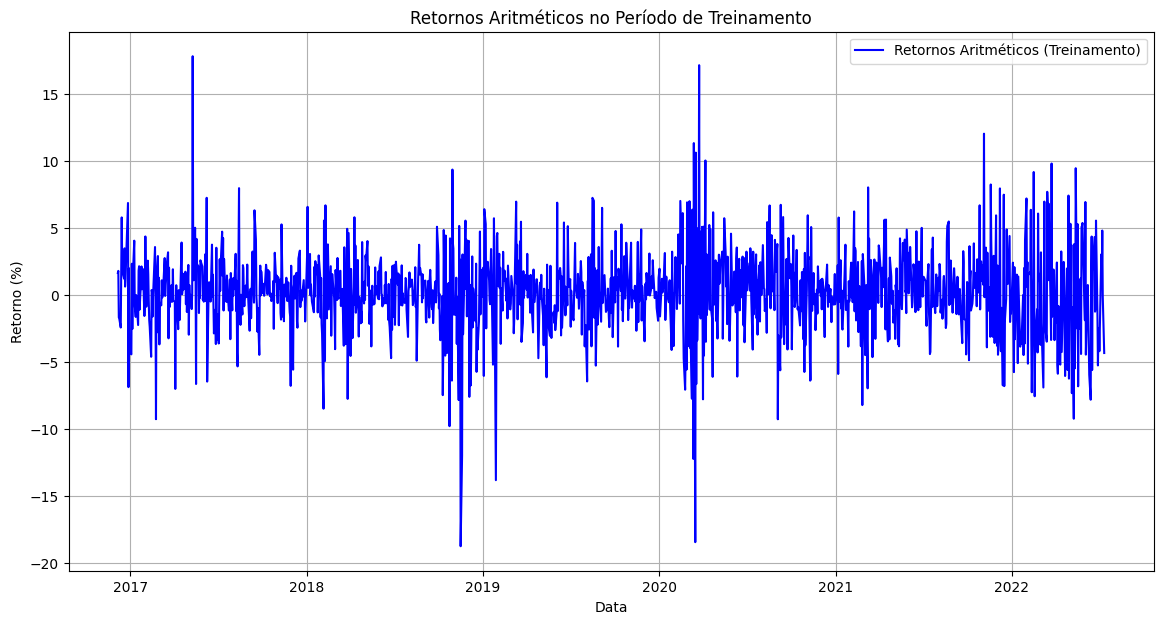
\includegraphics[width=\textwidth]{images/arit_retu_graph__train_data.png}
    \caption{Gráfico dos retornos aritméticos diários no período de treinamento.}
    \label{fig:retornos}
\end{figure}

\begin{figure}[H]
    \centering
    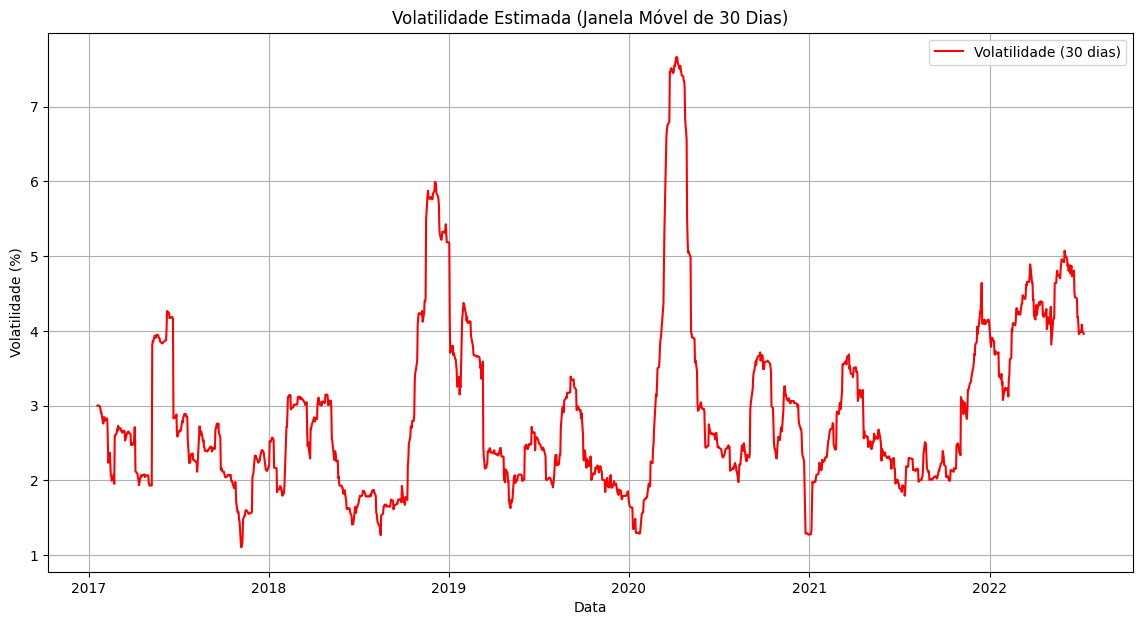
\includegraphics[width=\textwidth]{images/volatilidade_estimada.png}
    \caption{Volatilidade estimada com janela móvel de 30 dias.}
    \label{fig:volatilidade}
\end{figure}

\begin{figure}[H]
    \centering
    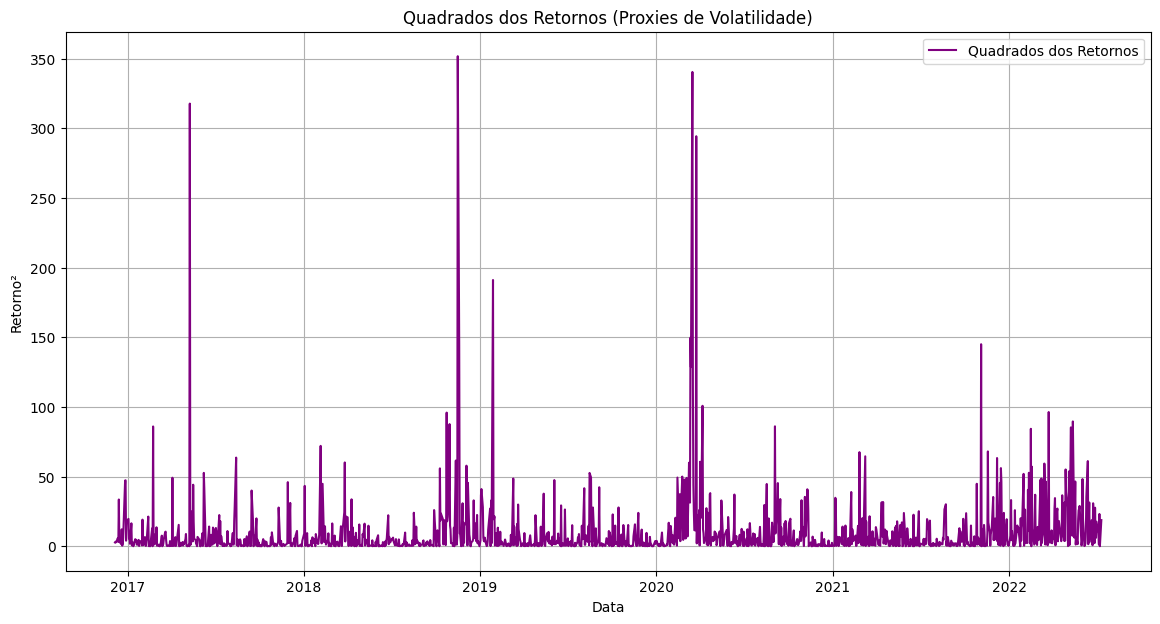
\includegraphics[width=\textwidth]{images/grafico_quadrados_retornos.png}
    \caption{Quadrados dos retornos como proxy de volatilidade.}
    \label{fig:quadrados}
\end{figure}



\subsubsection{Tabela com Estatísticas Descritivas}

Obtivemmos uma tabela com as seguintes estatísticas descritivas: mínimo, máximo, quantis 
de: 0.5\%, 1\%, 5\%, 50\%, 95\%, 99\%, 99.5\%; média, desvio padrão, assimetria e curtose.\\

Ao desenvolvermos e exercutarmos o código em Python para esta parte, obtivemos a saída apresentada na imagem \ref{fig:estat_desc}.

\begin{figure}[H]
    \centering
    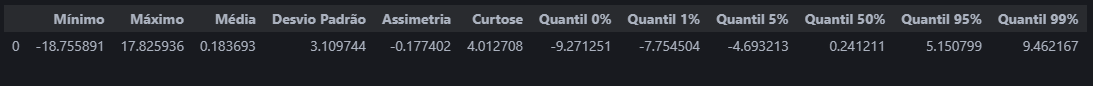
\includegraphics[width=\textwidth]{images/estat_desc.png}
    \caption{Saída do programa: estatísticas descritivas - Tarefa 1: pt.2}
    \label{fig:estat_desc}
\end{figure}


\paragraph{Análise das Estatísticas:}

\paragraph{Indicadores de Centralidade:}
\begin{itemize}
    \item \textbf{Média:} A média dos retornos diários é ligeiramente positiva (\(0.1837\%\)), indicando uma tendência geral de valorização da ação ao longo do período de treinamento.
    \item \textbf{Mediana (Quantil 50\%):} A mediana é \(0.2412\%\), ligeiramente superior à média, o que sugere uma leve assimetria negativa na distribuição.
\end{itemize}

\paragraph{Indicadores de Dispersão:}
\begin{itemize}
    \item \textbf{Desvio Padrão:} A volatilidade média é de \(3.1097\%\), refletindo a variabilidade dos retornos diários em torno da média.
    \item \textbf{Mínimo e Máximo:} Os extremos variam de uma perda de \(-18.7559\%\) a um ganho de \(17.8259\%\), evidenciando eventos extremos ocasionais.
    \item \textbf{Quantis:} Apenas \(0.5\%\) dos retornos são piores que \(-9.2713\%\), enquanto \(99.5\%\) estão abaixo de \(9.4622\%\), destacando a ocorrência de eventos extremos em ambas as caudas.
\end{itemize}

\paragraph{Indicadores de Forma da Distribuição:}
\begin{itemize}
    \item \textbf{Assimetria:} A assimetria negativa (\(-0.1774\)) indica que os retornos negativos extremos são mais frequentes ou intensos do que os positivos.
    \item \textbf{Curtose:} A curtose elevada (\(4.0127\)) indica uma distribuição leptocúrtica, com caudas mais pesadas do que em uma distribuição normal, reforçando a ocorrência de eventos extremos.
\end{itemize}

\paragraph{Interpretação Financeira:}

Os resultados sugerem que:
\begin{itemize}
    \item A ação da NVIDIA apresentou alta volatilidade no curto prazo, característica comum no setor de tecnologia, com eventos extremos destacados pelos quantis e pelos valores de mínimo e máximo.
    \item A distribuição dos retornos não é normal, como evidenciado pela assimetria e pela curtose, indicando a necessidade de modelos específicos para capturar os riscos extremos, como GARCH.
    \item A média positiva reflete uma tendência geral de crescimento, consistente com o desempenho da empresa no período.
\end{itemize}


\subsubsection{FAC e Teste LB para Dependência Linear}
Obtivemos a Função de Autocorrelação (FAC) e o teste de Ljung-Box (LB) para avaliar a dependência linear da série de retornos aritméticos no período de treinamento. Os resultados estão apresentados nas Figuras~\ref{fig:fac_retornos} e \ref{fig:lb_test}.

\paragraph{Análise da FAC (Figura~\ref{fig:fac_retornos}):}
O gráfico da FAC ilustra os coeficientes de autocorrelação para diferentes defasagens (\textit{lags}) na série de retornos aritméticos. As principais observações são:
\begin{itemize}
    \item \textbf{Defasagem 0:} Como esperado, a autocorrelação no lag 0 é igual a 1, representando a correlação perfeita da série consigo mesma.
    \item \textbf{Defasagens de 1 a 20:} A maioria dos coeficientes de autocorrelação está dentro dos intervalos de confiança (área sombreada azul), sugerindo que não há dependência linear significativa na série. 
    \item Apesar de algumas autocorrelações próximas ao limite do intervalo de confiança, elas podem ser atribuídas a flutuações aleatórias e não indicam correlação linear substancial.
\end{itemize}
De forma geral, os retornos aritméticos parecem ser linearmente independentes, o que é consistente com a hipótese de eficiência de mercado.

\paragraph{Teste de Ljung-Box (Figura~\ref{fig:lb_test}):}
Os resultados do teste de Ljung-Box para as primeiras 10 defasagens são apresentados na saída do programa. As métricas principais são:
\begin{itemize}
    \item \textbf{Estatística \(Q\):} O valor obtido foi \(54.881371\), indicando uma soma acumulada significativa de dependências ao longo das 10 primeiras defasagens.
    \item \textbf{Valor-p:} O valor-p associado foi extremamente pequeno (\(3.32335 \times 10^{-8}\)), permitindo rejeitar a hipótese nula de ausência de autocorrelação linear global. Isso sugere que, mesmo que as autocorrelações individuais sejam pequenas, há uma dependência linear acumulada ao longo das defasagens.
\end{itemize}

\paragraph{Conclusão:}
Apesar de o gráfico da FAC indicar pouca ou nenhuma dependência linear significativa em defasagens individuais, o teste de Ljung-Box detecta a existência de dependência linear acumulada até o lag 10. Isso implica que:
\begin{itemize}
    \item Modelos autoregressivos simples, como AR ou ARMA, podem capturar essas pequenas dependências lineares.
    \item No entanto, dado que as autocorrelações são geralmente fracas, o foco deve estar em modelos de variância condicional, como ARCH ou GARCH, para capturar a heterocedasticidade presente na série.
\end{itemize}

\begin{figure}[H]
    \centering
    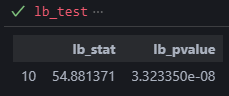
\includegraphics[scale=0.8]{images/lb_test.png}
    \caption{Saída do Programa - Estatísticas do Teste Ljung-Box (LB).}
    \label{fig:lb_test}
\end{figure}

\begin{figure}[H]
    \centering
    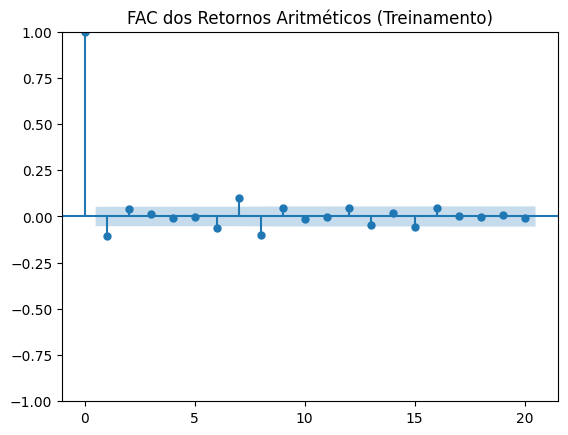
\includegraphics[scale=0.7]{images/fac_retornos.png}
    \caption{Gráfico da FAC dos Retornos Aritméticos.}
    \label{fig:fac_retornos}
\end{figure}


\subsubsection{FAC do Quadrado e Teste LB para Dependência Não-Linear}

Obtivemos a FAC dos quadrados dos retornos e o teste de Ljung-Box (LB) para avaliar a presença de dependência não-linear na série de retornos aritméticos. Os resultados estão apresentados nas Figuras~\ref{fig:fac_quadrados_retornos} e \ref{fig:lb_test_sq}.

\paragraph{Análise da FAC dos Quadrados dos Retornos (Figura~\ref{fig:fac_quadrados_retornos}):}
O gráfico da FAC dos quadrados dos retornos indica a autocorrelação entre os quadrados dos retornos ao longo de diferentes defasagens (lags). As observações principais são:
\begin{itemize}
    \item \textbf{Defasagem 0 (Lag 0):} O coeficiente de autocorrelação no lag 0 é igual a 1, como esperado, representando a correlação perfeita da série consigo mesma.
    \item \textbf{Defasagens de 1 a 20:} Diversos coeficientes de autocorrelação estão fora do intervalo de confiança (área sombreada azul), indicando a presença de dependências não-lineares significativas. Essa evidência aponta para a existência de clusters de volatilidade, nos quais períodos de alta volatilidade são seguidos por alta volatilidade, e períodos de baixa volatilidade são seguidos por baixa volatilidade.
\end{itemize}
\textbf{Conclusão da FAC:} A análise da FAC confirma a presença de heterocedasticidade condicional na série de retornos, ou seja, a variância dos retornos não é constante ao longo do tempo. Este é um comportamento típico de séries financeiras.

\paragraph{Resultados do Teste de Ljung-Box (Figura~\ref{fig:lb_test_sq}):}
O teste de Ljung-Box foi aplicado para investigar a dependência não-linear acumulada nos quadrados dos retornos até o lag 10. As métricas principais obtidas foram:
\begin{itemize}
    \item \textbf{Estatística \(Q\):} O valor calculado foi \(277.566594\), indicando uma forte evidência de dependência não-linear.
    \item \textbf{Valor-p:} O valor-p associado foi \(8.490328 \times 10^{-54}\), que é extremamente pequeno, permitindo rejeitar a hipótese nula de ausência de dependência não-linear.
\end{itemize}
\textbf{Conclusão do Teste LB:} Os resultados do teste confirmam que há dependências não-lineares significativas na série de retornos, como esperado em séries financeiras.

\paragraph{Implicações Financeiras:}
A presença de dependências não-lineares e clusters de volatilidade tem implicações importantes:
\begin{itemize}
    \item **Clusters de Volatilidade:** Períodos de alta volatilidade persistem por algum tempo antes de retornarem a níveis mais baixos, e o mesmo ocorre para períodos de baixa volatilidade.
    \item **Modelagem Apropriada:** A presença de heterocedasticidade condicional torna os modelos ARCH (Autoregressive Conditional Heteroskedasticity) e GARCH (Generalized ARCH) mais adequados para modelar a série.
    \item **Gestão de Riscos:** A dependência não-linear implica que a volatilidade futura pode ser parcialmente previsível com base no comportamento recente, o que é crucial para estratégias de precificação de ativos e gestão de portfólios.
\end{itemize}

\begin{figure}[H]
    \centering
    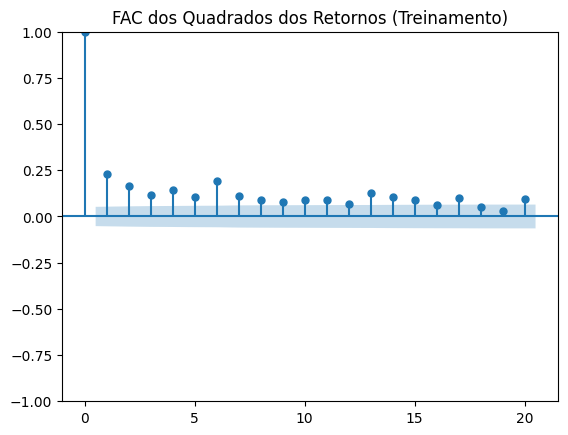
\includegraphics[scale=0.7]{images/fac_quadrados_retornos.png}
    \caption{Gráfico da FAC dos Quadrados dos Retornos Aritméticos.}
    \label{fig:fac_quadrados_retornos}
\end{figure}

\begin{figure}[H]
    \centering
    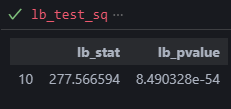
\includegraphics[scale=0.7]{images/lb_test_sq.png}
    \caption{Saída do Programa: LB Teste para Dependência Não-Linear.}
    \label{fig:lb_test_sq}
\end{figure}


\subsubsection{Teste ARCH}

Obtivemos o teste ARCH para avaliar a presença de heterocedasticidade condicional na série de retornos. Os resultados estão apresentados na Figura~\ref{fig:teste_ARCH}.

\paragraph{Hipóteses do Teste ARCH:}
\begin{itemize}
    \item \textbf{Hipótese Nula (\(H_0\)):} Não há heterocedasticidade condicional, ou seja, a variância dos resíduos é constante ao longo do tempo (homocedasticidade).
    \item \textbf{Hipótese Alternativa (\(H_1\)):} Há heterocedasticidade condicional, indicando que a variância dos resíduos depende de informações passadas.
\end{itemize}

\paragraph{Resultados do Teste:}
\begin{itemize}
    \item \textbf{Estatística LM (Lagrange Multiplier):} O valor obtido foi \( 139.0313 \), o que representa uma evidência significativa de heterocedasticidade condicional.
    \item \textbf{Valor-p:} O valor-p associado foi \( 6.65576 \times 10^{-25} \), que é extremamente pequeno e muito menor que os níveis de significância usuais (\( \alpha = 0.01, 0.05 \)).
\end{itemize}

\paragraph{Interpretação dos Resultados:}
\begin{itemize}
    \item Dado o valor-p muito pequeno, rejeitamos a hipótese nula (\(H_0\)) com alto grau de confiança, concluindo que há heterocedasticidade condicional na série.
    \item Essa evidência sugere que a variância dos resíduos não é constante ao longo do tempo, mas sim dependente de informações passadas, um comportamento comum em séries financeiras.
\end{itemize}

\paragraph{Implicações Financeiras e Práticas:}
\begin{itemize}
    \item \textbf{Modelagem Apropriada:} A presença de heterocedasticidade condicional torna modelos como ARCH (Autoregressive Conditional Heteroskedasticity) e GARCH (Generalized ARCH) mais adequados para descrever a dinâmica da série.
    \item \textbf{Previsão de Volatilidade:} A heterocedasticidade condicional indica que a volatilidade futura pode ser prevista com base na variância passada, o que é crucial para estratégias de precificação de ativos e gestão de riscos.
    \item \textbf{Gestão de Riscos:} A identificação de clusters de volatilidade permite que gestores e investidores ajustem suas estratégias para períodos de maior ou menor risco.
\end{itemize}

\begin{figure}[H]
    \centering
    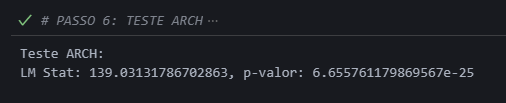
\includegraphics[scale=0.7]{images/teste_ARCH.png}
    \caption{Saída do Programa: Teste ARCH.}
    \label{fig:teste_ARCH}
\end{figure}


\subsubsection{Histograma, Q-Q Plot e Teste de Normalidade}

A análise de normalidade da série de retornos aritméticos foi conduzida por meio do Histograma, do Q-Q Plot e do Teste de Normalidade (Shapiro-Wilk). A seguir, apresentamos a descrição detalhada dos resultados.

\begin{figure}[H]
    \centering
    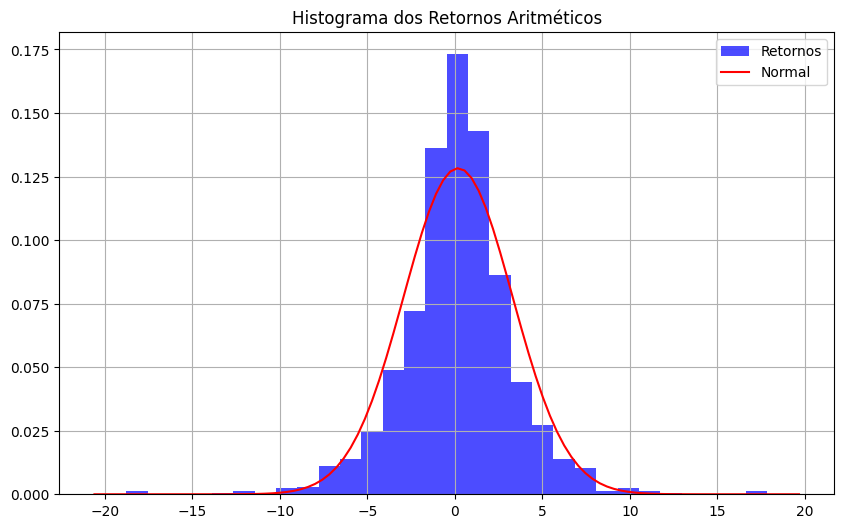
\includegraphics[scale=0.7]{images/histograma.png}
    \caption{Histograma dos Retornos Aritméticos.}
    \label{fig:histograma}
\end{figure}

\textbf{Histograma:} Na Figura~\ref{fig:histograma}, observa-se a distribuição empírica dos retornos, sobreposta a uma curva de densidade teórica da distribuição normal (linha vermelha). Embora a parte central da distribuição esteja próxima da normalidade, há caudas mais pesadas, indicando a presença de eventos extremos, comuns em séries financeiras. Esses eventos extremos sugerem maior frequência de retornos extremos (positivos e negativos) do que o esperado sob a hipótese de normalidade.

\begin{figure}[H]
    \centering
    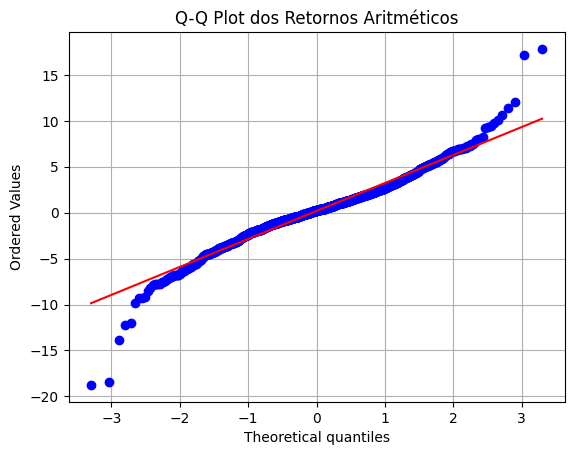
\includegraphics[scale=0.7]{images/qqplot.png}
    \caption{Q-Q Plot dos Retornos Aritméticos.}
    \label{fig:qqplot}
\end{figure}

\textbf{Q-Q Plot:} A Figura~\ref{fig:qqplot} apresenta o Q-Q Plot, que compara os quantis empíricos dos dados com os quantis de uma distribuição normal teórica. A maior parte dos pontos está alinhada com a linha vermelha, indicando proximidade à normalidade na região central da distribuição. No entanto, os desvios observados nas extremidades confirmam a presença de caudas mais pesadas, caracterizando maior frequência de eventos extremos do que o esperado em uma distribuição normal.

\begin{figure}[H]
    \centering
    
\includegraphics[scale=0.7]{images/teste_normalidade.png}
    \caption{Saída do Programa: Teste de Normalidade (Shapiro-Wilk).}
    \label{fig:teste_norm}
\end{figure}

\textbf{Teste de Normalidade (Shapiro-Wilk):} O teste Shapiro-Wilk foi utilizado para formalizar a avaliação da normalidade. Os resultados são os seguintes:
\begin{itemize}
    \item Estatística \( W = 0.9598 \);
    \item Valor-p \( = 2.9257 \times 10^{-19} \).
\end{itemize}

Com um valor-p extremamente pequeno (\(< 0.05\)), rejeitamos a hipótese nula de que os dados seguem uma distribuição normal. Isso confirma as observações visuais do histograma e do Q-Q Plot, reforçando que os retornos não são normalmente distribuídos e apresentam caudas mais pesadas.\\

Entçao, os resultados indicam que:
\begin{itemize}
    \item Os retornos aritméticos não seguem uma distribuição normal.
    \item A distribuição apresenta caudas mais pesadas, típicas de séries financeiras.
    \item Modelos baseados em pressupostos de normalidade podem não ser adequados para capturar a dinâmica dos retornos.
\end{itemize}
Portanto, sugere-se o uso de modelos alternativos, como distribuições t-student ou modelos de volatilidade, para melhor representação estatística da série.




\section{TAREFA 2: Modelos GARCH para séries de retornos financeiros}

Nesta seção, devemos ajustar e avaliar modelos GARCH (p, q) para modelar a volatilidade condicional dos retornos aritméticos. O objetivo é capturar a dinâmica da variância condicional dos retornos financeiros utilizando modelos GARCH. Como a autocorrelação nos retornos aritméticos é desprezível, presume-se que a média condicional dos retornos seja constante.

\subsection{Divisão dos Dados}
Para realizar as análises, a série de retornos será dividida em dois períodos distintos:
\begin{itemize}
    \item \textbf{Período de Treinamento}: 70\% da série de retornos aritméticos, que será utilizado para estimar os parâmetros dos modelos GARCH.
    \item \textbf{Período de Teste}: 30\% da série de retornos aritméticos, utilizado para avaliar a adequação e a performance dos modelos ajustados.
\end{itemize}

\subsection{Modelos a Serem Ajustados}
Dois modelos GARCH (p, q) serão ajustados:
\begin{enumerate}
    \item \textbf{Modelo GARCH com distribuição normal \(N(0,1)\)}:
    \begin{itemize}
        \item Assume que os resíduos padronizados do modelo seguem uma distribuição normal padrão \(N(0,1)\).
        \item Este modelo será usado como base para avaliar a adequação da normalidade nos resíduos.
    \end{itemize}
    \item \textbf{Modelo GARCH com distribuição t-Student \(t(0,1,m)\)}:
    \begin{itemize}
        \item Este modelo é indicado quando há presença de excesso de curtose nos resíduos padronizados.
        \item O parâmetro \(m\), que representa o grau de liberdade da distribuição t-Student, será estimado em conjunto com os parâmetros \(p\) e \(q\).
    \end{itemize}
\end{enumerate}

\subsection{Objetivos da Análise}
Os principais objetivos da tarefa são:
\begin{itemize}
    \item \textbf{Capturar a dinâmica da variância condicional}: Identificar a estrutura mais adequada do modelo GARCH (p, q) para os dados analisados.
    \item \textbf{Avaliar os resíduos}: Verificar se os resíduos padronizados apresentam comportamento consistente com as suposições feitas, como a ausência de autocorrelação e a aderência às distribuições \(N(0,1)\) e \(t(0,1,m)\).
    \item \textbf{Comparar os modelos}: Comparar os resultados obtidos com as duas distribuições de erro e identificar qual modelo fornece melhor ajuste aos dados.
\end{itemize}

\subsection{Excesso de Curtose e Escolha do Modelo}
Durante a análise, é esperado que o modelo com distribuição \(N(0,1)\) apresente resíduos com excesso de curtose, indicando que os dados não seguem uma distribuição normal. Para lidar com essa característica, o modelo GARCH com distribuição t-Student \(t(0,1,m)\) será ajustado, pois:
\begin{itemize}
    \item A distribuição \(t(0,1,m)\) possui caudas mais pesadas, sendo mais adequada para séries com alta volatilidade e extremos.
    \item A curtose dessa distribuição é definida por \(k = 3 + 6/(m-4)\), onde \(m\) será estimado com base nos dados.
\end{itemize}

 Espera-se que o modelo com distribuição t-Student \(t(0,1,m)\) apresente melhores resultados em séries com excesso de curtose e volatilidade elevada.
O ajuste adequado do modelo GARCH permitirá identificar a dinâmica de variância condicional e capturar eventos extremos observados na série.



\subsection{Parte I}\label{subsec:tarefa2_pt1}

Nesta seção\footnote{Os códigos Python utilizados nesta seção estão disponíveis em \ref{apendice:codigo_tarefa2_pt1}}, analisamos os melhores modelos GARCH(p, q) utilizando os critérios de seleção AIC e BIC. Avaliamos os ajustes para distribuições normais \(N(0,1)\) e t-student \(t(0,1,m)\), com \(m\) sendo o grau de liberdade estimado. Abaixo detalhamos os resultados de forma científica e explicativa.

\subsubsection{Critério AIC}

O critério AIC (\textit{Akaike Information Criterion}) penaliza modelos mais complexos, mas é mais permissivo do que o BIC. Observamos os modelos com menor AIC para cada distribuição:

\begin{itemize}
    \item \textbf{Distribuição Normal (\(N(0,1)\)}:
        \begin{itemize}
            \item Melhor modelo: GARCH(2, 2).
            \item Parâmetros estimados:
            \begin{itemize}
                \item \(\mu = 0.312423\), \(\omega = 1.486483\),
                \item \(\alpha_1 = 0.082336\), \(\alpha_2 = 0.194209\),
                \item \(\beta_1 = 0.000000\), \(\beta_2 = 0.574771\).
            \end{itemize}
        \end{itemize}
    \item \textbf{Distribuição \(t(0,1,m)\)}:
        \begin{itemize}
            \item Melhor modelo: GARCH(1, 1).
            \item Parâmetros estimados:
            \begin{itemize}
                \item \(\mu = 0.265515\), \(\omega = 0.429776\),
                \item \(\alpha_1 = 0.141756\), \(\beta_1 = 0.823232\),
                \item \(\nu = 5.409048\) (grau de liberdade).
            \end{itemize}
        \end{itemize}
\end{itemize}

\begin{figure}[H]
    \centering
    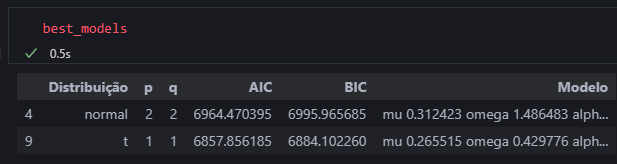
\includegraphics[scale=0.7]{images/best_models_AIC.png}
    \caption{Saída do Programa - melhores modelos AIC.}
    \label{fig:best_models_AIC}
\end{figure}

\subsubsection{Critério BIC}

O critério BIC (\textit{Bayesian Information Criterion}) é mais conservador, penalizando mais severamente a complexidade do modelo. Os resultados são:

\begin{itemize}
    \item \textbf{Distribuição Normal (\(N(0,1)\)}:
        \begin{itemize}
            \item Melhor modelo: GARCH(1, 1).
            \item Parâmetros estimados:
            \begin{itemize}
                \item \(\mu = 0.273855\), \(\omega = 0.680002\),
                \item \(\alpha_1 = 0.000000\), \(\beta_1 = 0.000000\).
            \end{itemize}
        \end{itemize}
    \item \textbf{Distribuição \(t(0,1,m)\)}:
        \begin{itemize}
            \item Melhor modelo: GARCH(1, 1).
            \item Parâmetros estimados:
            \begin{itemize}
                \item \(\mu = 0.265515\), \(\omega = 0.429776\),
                \item \(\alpha_1 = 0.141756\), \(\beta_1 = 0.823232\),
                \item \(\nu = 5.409048\).
            \end{itemize}
        \end{itemize}
\end{itemize}

\begin{figure}[H]
    \centering
    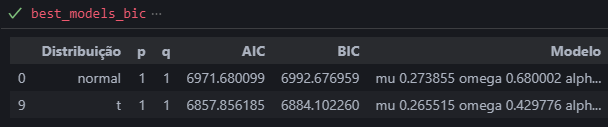
\includegraphics[scale=0.7]{images/best_models_BIC.png}
    \caption{Saída do Programa - melhores modelos BIC.}
    \label{fig:best_models_BIC}
\end{figure}

\subsubsection{Parâmetros para as Equações dos Modelos}

Os parâmetros estimados dos modelos selecionados permitem descrever as equações das variâncias condicionais como segue:

\begin{itemize}
    \item \textbf{GARCH(2, 2) com distribuição normal (\(N(0,1)\)}:
    \[
    \sigma_t^2 = 1.486483 + 0.082336 \epsilon_{t-1}^2 + 0.194209 \epsilon_{t-2}^2 + 0.574771 \sigma_{t-2}^2
    \]
    \item \textbf{GARCH(1, 1) com distribuição t-student (\(t(0,1,m)\))}:
    \[
    \sigma_t^2 = 0.429776 + 0.141756 \epsilon_{t-1}^2 + 0.823232 \sigma_{t-1}^2
    \]
\end{itemize}

\begin{figure}[H]
    \centering
    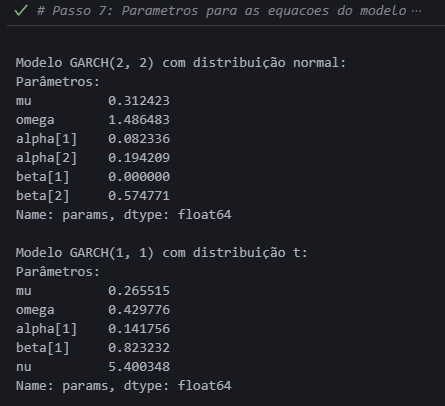
\includegraphics[scale=0.8]{images/parametros_para_equacoes.png}
    \caption{Saída do Programa - parâmetros estimados para as equações.}
    \label{fig:parametros_para_equacoes}
\end{figure}

\subsubsection{Discussão}

Os modelos com distribuição \(t(0,1,m)\) se destacaram em ambos os critérios AIC e BIC, reforçando sua capacidade de capturar características estilizadas como o excesso de curtose. No entanto, para a distribuição normal, o modelo GARCH(1, 1) é preferível pela simplicidade, enquanto o GARCH(2, 2) é mais adequado ao critério AIC, indicando melhor ajuste relativo.

\subsubsection{Equações dos Modelos GARCH}

Os modelos GARCH (\textit{Generalized Autoregressive Conditional Heteroskedasticity}) são amplamente utilizados para modelar a volatilidade condicional em séries temporais financeiras. A forma genérica do modelo GARCH(p, q) é dada por:

\begin{equation}
    \sigma_t^2 = \omega + \sum_{i=1}^p \alpha_i \epsilon_{t-i}^2 + \sum_{j=1}^q \beta_j \sigma_{t-j}^2,
    \label{eq:garch_general}
\end{equation}

onde:
\begin{itemize}
    \item \(\sigma_t^2\) é a variância condicional no tempo \(t\),
    \item \(\omega > 0\) é o termo constante,
    \item \(\alpha_i \geq 0\) são os coeficientes associados aos choques anteriores (\(\epsilon_{t-i}^2\)),
    \item \(\beta_j \geq 0\) são os coeficientes associados às variâncias condicionais defasadas (\(\sigma_{t-j}^2\)),
    \item \(p\) é o número de termos ARCH (choques passados),
    \item \(q\) é o número de termos GARCH (volatilidades passadas).
\end{itemize}

Abaixo estão as especificações detalhadas das variâncias condicionais para os melhores modelos estimados.

\paragraph{Modelo GARCH(2, 2) com distribuição \( N(0,1) \):}
\begin{equation}
    \sigma_t^2 = 1.486483 + 0.082336 \cdot \epsilon_{t-1}^2 + 0.194209 \cdot \epsilon_{t-2}^2 + 0.574771 \cdot \sigma_{t-2}^2
    \label{eq:garch_normal}
\end{equation}

\paragraph{Modelo GARCH(1, 1) com distribuição \( t(0,1,m) \):}
\begin{equation}
    \sigma_t^2 = 0.429776 + 0.141756 \cdot \epsilon_{t-1}^2 + 0.823232 \cdot \sigma_{t-1}^2
    \label{eq:garch_student}
\end{equation}


Os modelos acima capturam a variância condicional da série de retornos, ajustando-se bem às respectivas distribuições \( N(0,1) \) e \( t(0,1,m) \). 
Os coeficientes \(\alpha_i\) e \(\beta_j\) indicam a persistência dos choques e da variância condicional passada, respectivamente. O modelo com distribuição \(t(0,1,m)\) acomoda melhor os dados devido à sua maior flexibilidade para lidar com excesso de curtose, conforme observado nos retornos financeiros analisados.



\subsection{Parte II: Testes de Diagnóstico nos Resíduos Padronizados}\label{subsec:tarefa2_pt2}

Nesta parte\footnote{Códigos Python para esta parte disponíveis em \ref{apendice:codigo_tarefa2_pt2}.}, avaliamos os resíduos padronizados dos melhores modelos selecionados na Parte I. Realizamos os seguintes testes: 
\begin{itemize}
    \item FAC dos resíduos padronizados;
    \item FAC dos quadrados dos resíduos padronizados;
    \item Teste ARCH;
    \item Q-Q Plot e Teste Jarque-Bera.
\end{itemize}

Além disso, avaliamos a adequação dos modelos com base nos resultados e consideramos ajustes para possíveis reespecificações. Abaixo estão os passos e resultados detalhados para cada teste.

\subsubsection{Parte (a): FAC dos Resíduos Padronizados}

Nesta subseção, analisamos os gráficos da Função de Autocorrelação (FAC) dos resíduos padronizados para verificar a presença de dependência linear residual nos modelos ajustados.

\paragraph{FAC dos Resíduos Padronizados - Normal:}

\begin{figure}[H]
    \centering
    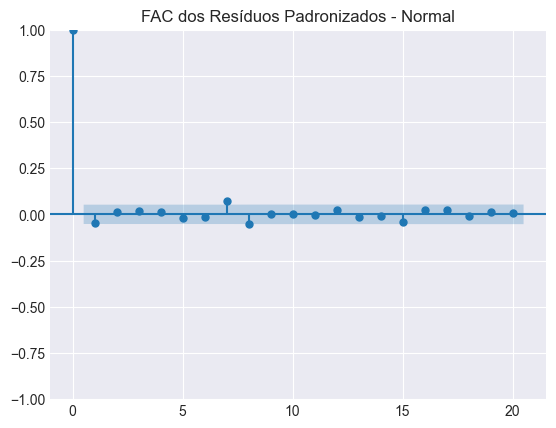
\includegraphics[scale=0.7]{images/FAC_resid_padronizados_NORMAL_tarefa2pt2.png}
    \caption{FAC dos resíduos padronizados - Normal.}
    \label{fig:FAC_resid_padronizados_NORMAL_tarefa2pt2}
\end{figure}

No gráfico da FAC dos resíduos padronizados ajustados com a distribuição normal, observa-se:
\begin{itemize}
    \item O coeficiente de autocorrelação para o primeiro lag está próximo de 1, como esperado, dado que os resíduos padronizados são derivados diretamente do modelo ajustado.
    \item Para os lags subsequentes, os coeficientes permanecem dentro dos intervalos de confiança (\(\pm 1.96 / \sqrt{n}\)), indicando ausência de autocorrelação significativa.
\end{itemize}

Este resultado sugere que o modelo GARCH(2,2) com distribuição \(N(0,1)\) capturou adequadamente a volatilidade condicional, deixando os resíduos padronizados livres de dependência linear.

\paragraph{FAC dos Resíduos Padronizados - T:}

\begin{figure}[H]
    \centering
    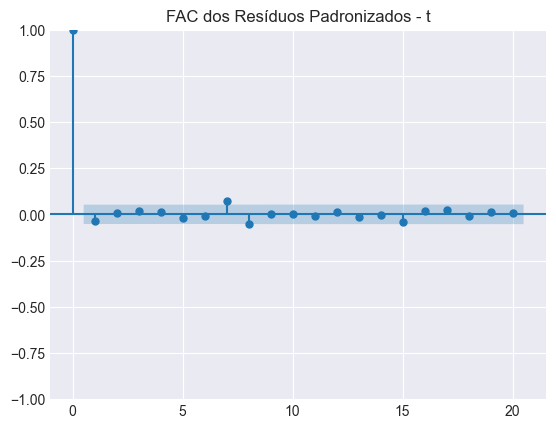
\includegraphics[scale=0.7]{images/FAC_resid_padronizados_T_tarefa2pt2.png}
    \caption{FAC dos resíduos padronizados - T.}
    \label{fig:FAC_resid_padronizados_T_tarefa2pt2}
\end{figure}

No gráfico da FAC dos resíduos padronizados ajustados com a distribuição \(t(0,1,m)\), observa-se:
\begin{itemize}
    \item O coeficiente de autocorrelação para o primeiro lag também está próximo de 1.
    \item Nos lags subsequentes, os coeficientes permanecem dentro dos intervalos de confiança, indicando ausência de autocorrelação significativa.
\end{itemize}

A utilização da distribuição \(t\) permite capturar características como curtose elevada, o que pode ser observado na robustez dos resíduos padronizados ajustados. O modelo GARCH(1,1) com distribuição \(t\) mostrou-se adequado para modelar a volatilidade condicional da série.\\

Ambos os modelos (GARCH com distribuições \(N(0,1)\) e \(t(0,1,m)\)) apresentam resultados semelhantes em termos de ausência de autocorrelação nos resíduos padronizados, sugerindo que ambos capturam adequadamente a estrutura de dependência linear da série de retornos. Contudo, análises complementares, como dependência não-linear e normalidade, são necessárias para uma avaliação completa.


\subsubsection{Parte (b): FAC dos Quadrados dos Resíduos Padronizados}

A análise da FAC dos quadrados dos resíduos padronizados é crucial para avaliar a presença de heterocedasticidade condicional remanescente nos resíduos dos modelos ajustados. Abaixo estão as interpretações detalhadas dos resultados apresentados nos gráficos para as distribuições \(N(0,1)\) e \(t(0,1,m)\).

\begin{figure}[H]
    \centering
    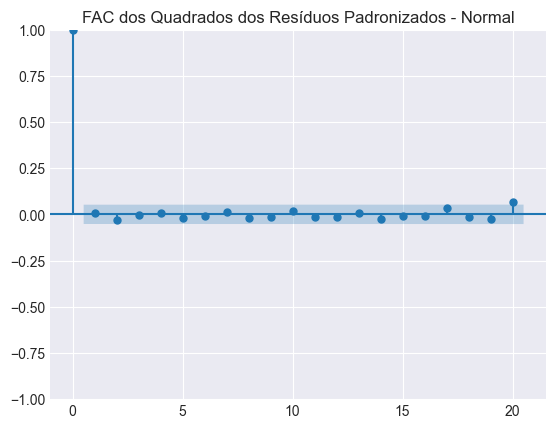
\includegraphics[scale=0.7]{images/FAC_quadrados_resid_padronizados_Normal_tarefa2pt2.png}
    \caption{FAC dos quadrados dos resíduos padronizados - Normal.}
    \label{fig:FAC_quadrados_resid_padronizados_Normal_tarefa2pt2}
\end{figure}

\begin{figure}[H]
    \centering
    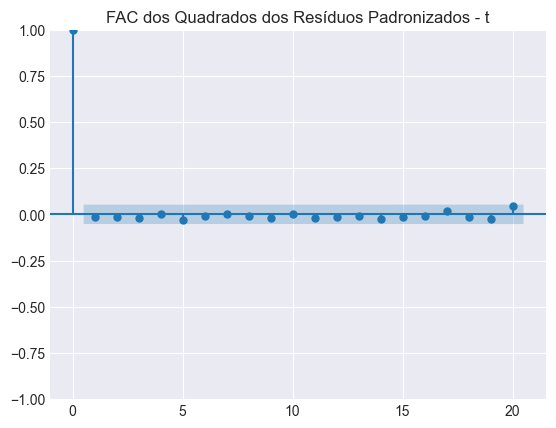
\includegraphics[scale=0.7]{images/FAC_quadrados_resid_padronizados_T_tarefa2pt2.png}
    \caption{FAC dos quadrados dos resíduos padronizados - T.}
    \label{fig:FAC_quadrados_resid_padronizados_T_tarefa2pt2}
\end{figure}


\paragraph{Modelo com Distribuição \(N(0,1)\}:}
\begin{itemize}
    \item \textbf{Observações Gerais:} O gráfico apresenta um pico inicial em \( \text{lag } 0\), o que é esperado, pois corresponde à autocorrelação da série consigo mesma. Nos lags subsequentes (\(1\) em diante), as autocorrelações estão dentro dos limites de confiança, sugerindo que o modelo capturou bem a maior parte da heterocedasticidade condicional.
    \item \textbf{Interpretação Estatística:} 
    \begin{itemize}
        \item A ausência de autocorrelações significativas para \( \text{lag} > 0\) indica que o modelo \(GARCH(2,2)\) com distribuição \(N(0,1)\) conseguiu capturar os clusters de volatilidade na maior parte da série.
    \end{itemize}
    \item \textbf{Conclusão:} O modelo apresenta bom ajuste, sem indícios relevantes de heterocedasticidade remanescente nos resíduos padronizados.
\end{itemize}

\paragraph{Modelo com Distribuição \(t(0,1,m)\}:}
\begin{itemize}
    \item \textbf{Observações Gerais:} Assim como no modelo \(N(0,1)\), há um pico inicial em \( \text{lag } 0\), que é esperado. Para os lags subsequentes, as autocorrelações estão dentro dos intervalos de confiança.
    \item \textbf{Interpretação Estatística:} 
    \begin{itemize}
        \item A adequação do modelo \(GARCH(1,1)\) com distribuição \(t(0,1,m)\) é evidenciada pela ausência de autocorrelações significativas nos lags \(1\) e superiores.
        \item A flexibilidade da distribuição \(t\) ajuda a modelar séries com caudas pesadas, resultando em resíduos mais próximos de um comportamento branco (sem autocorrelações significativas).
    \end{itemize}
    \item \textbf{Conclusão:} Este modelo mostrou um desempenho ligeiramente superior, capturando a estrutura de dependência na volatilidade condicional de forma eficiente.
\end{itemize}

\paragraph{Comparação Geral:}
\begin{itemize}
    \item Ambos os modelos mostraram resultados satisfatórios, sem autocorrelações significativas para \( \text{lag} > 0\).
    \item O modelo com distribuição \(t(0,1,m)\) teve desempenho ligeiramente superior, provavelmente devido à maior flexibilidade da distribuição em capturar padrões de heterocedasticidade.
\end{itemize}







\subsubsection{Parte (c): Teste ARCH}

O teste ARCH foi aplicado para avaliar a presença de heterocedasticidade adicional nos resíduos padronizados dos modelos ajustados. Este teste verifica se há variação condicional não explicada, que poderia indicar inadequação do modelo para capturar a dinâmica da variância condicional. \\

Os resultados do teste ARCH estão apresentados na Tabela \ref{tab:teste_arch}, e a saída do programa ao executar o teste está ilustrada na Figura \ref{fig:teste_ARCH_tarefa2_pt2}.

\begin{figure}[H]
    \centering
    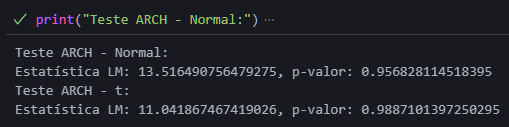
\includegraphics[scale=0.7]{images/teste_ARCH_tarefa2_pt2.png}
    \caption{Saída do programa: Teste ARCH.}
    \label{fig:teste_ARCH_tarefa2_pt2}
\end{figure}

\begin{itemize}
    \item \textbf{\(H_0\):} Os resíduos são homocedásticos, ou seja, não há heterocedasticidade condicional adicional.
    \item \textbf{\(H_a\):} Os resíduos apresentam heterocedasticidade condicional adicional.
    \item \textbf{Estatística de teste:} Lagrange Multiplier (LM).
    \item \textbf{Distribuição:} A estatística LM segue uma distribuição qui-quadrado (\(\chi^2\)) sob \(H_0\).
    \item \textbf{Nível de significância:} \(\alpha = 0.05\).
\end{itemize}

\begin{table}[H]
    \centering
    \caption{Resultados do Teste ARCH.}
    \label{tab:teste_arch}
    \begin{tabular}{ccc}
        \hline
        \textbf{Modelo} & \textbf{Estatística LM} & \textbf{p-valor} \\
        \hline
        GARCH(2, 2) - \(N(0,1)\) & \(13.516\) & \(0.9568\) \\
        GARCH(1, 1) - \(t(0,1,m)\) & \(11.042\) & \(0.9887\) \\
        \hline
    \end{tabular}
\end{table}

\textbf{Interpretação dos Resultados:}
\begin{itemize}
    \item Para ambos os modelos, os p-valores são significativamente maiores que o nível de significância \(\alpha = 0.05\), indicando que não há evidências estatísticas para rejeitar \(H_0\). 
    \item Isso sugere que os resíduos dos modelos ajustados são homocedásticos, ou seja, não apresentam heterocedasticidade condicional remanescente.
    \item O modelo GARCH(1, 1) com distribuição \(t(0,1,m)\) apresentou um p-valor ligeiramente maior (\(0.9887\)) do que o modelo GARCH(2, 2) com distribuição \(N(0,1)\) (\(0.9568\)), o que pode indicar uma melhor adequação aos dados.
    \item A ausência de heterocedasticidade remanescente reforça a adequação dos modelos ajustados para capturar a dinâmica de volatilidade condicional dos retornos financeiros.
\end{itemize}


\subsubsection{Parte (d): Q-Q Plot e Teste Jarque-Bera}
Os resíduos padronizados dos modelos foram avaliados quanto à normalidade utilizando Q-Q Plots e o Teste Jarque-Bera. Os gráficos para cada modelo estão nas Figuras \ref{fig:qqplot_normal} e \ref{fig:qqplot_t}. A Tabela \ref{tab:teste_jb} apresenta os resultados do Teste Jarque-Bera.

\paragraph{Q-Q Plots:}
Os Q-Q Plots permitem uma avaliação visual da adequação dos resíduos padronizados a uma distribuição teórica. 

\begin{itemize}
    \item \textbf{Modelo \(N(0,1)\):} Como mostrado na Figura \ref{fig:qqplot_normal}, observa-se um alinhamento razoável dos pontos à linha reta para os valores centrais. No entanto, há desvios significativos nas caudas, indicando que os resíduos apresentam caudas mais pesadas do que o esperado sob uma distribuição normal.
    \item \textbf{Modelo \(t(0,1,m)\):} Na Figura \ref{fig:qqplot_t}, o alinhamento dos pontos à linha reta é mais consistente, inclusive nas caudas. Isso evidencia que o modelo com distribuição \(t\) captura melhor a curtose elevada dos resíduos padronizados.
\end{itemize}

\paragraph{Teste Jarque-Bera (JB):}
O Teste Jarque-Bera foi utilizado para avaliar quantitativamente a normalidade dos resíduos. Os resultados estão resumidos na Tabela \ref{tab:teste_jb}, harmonizando os resultados visualizados da saída do programa na imagem \ref{fig:teste_JB_tarefa2pt2}.

\begin{figure}[H]
    \centering
    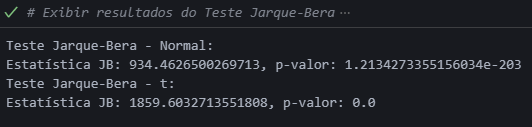
\includegraphics[scale=0.7]{images/teste_JB_tarefa2pt2.png}
    \caption{Saída do programa: Teste Jarque-Bera.}
    \label{fig:teste_JB_tarefa2pt2}
\end{figure}


\begin{itemize}
    \item \(H_0\): Os resíduos seguem uma distribuição normal.
    \item \(H_a\): Os resíduos não seguem uma distribuição normal.
\end{itemize}

\begin{figure}[H]
    \centering
    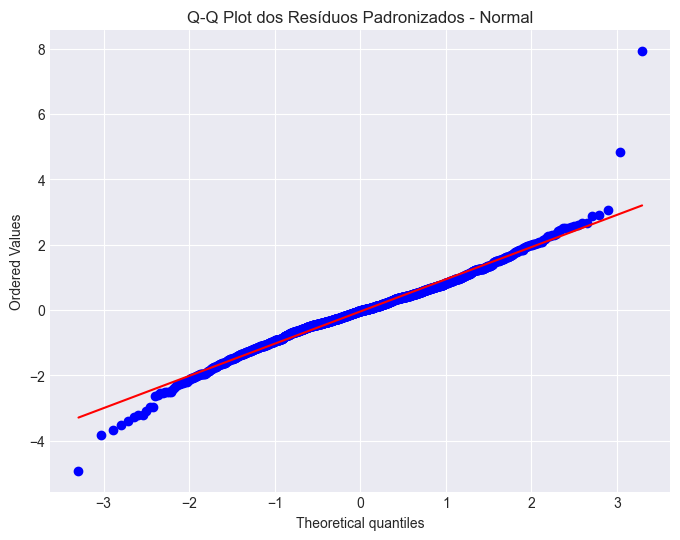
\includegraphics[scale=0.7]{images/QQplot_residuos_padronizados_Normal_tarefa2pt2.png}
    \caption{Q-Q Plot - \(N(0,1)\).}
    \label{fig:qqplot_normal}
\end{figure}

\begin{figure}[H]
    \centering
    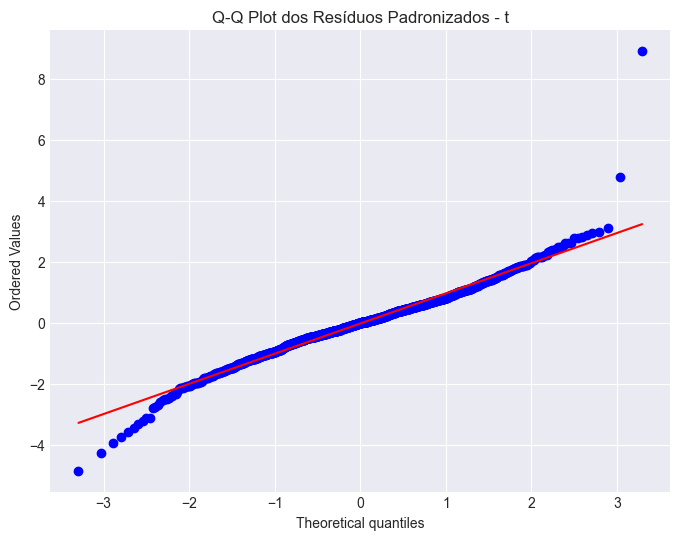
\includegraphics[scale=0.7]{images/QQplot_residuos_padronizados_T_tarefa2pt2.png}
    \caption{Q-Q Plot - \(t(0,1,m)\).}
    \label{fig:qqplot_t}
\end{figure}

\begin{table}[H]
    \centering
    \caption{Resultados do Teste Jarque-Bera.}
    \label{tab:teste_jb}
    \begin{tabular}{cccc}
        \hline
        \textbf{Modelo} & \textbf{Estatística JB} & \textbf{p-valor} & \textbf{Conclusão} \\
        \hline
        GARCH(2, 2) - \(N(0,1)\) & 934.44 & \(1.22 \times 10^{-203}\) & Rejeita \(H_0\) \\
        GARCH(1, 1) - \(t(0,1,m)\) & 1859.55 & 0.0 & Rejeita \(H_0\) \\
        \hline
    \end{tabular}
\end{table}

\paragraph{Interpretação:}
Os resultados do Teste Jarque-Bera indicam que ambos os modelos apresentam resíduos padronizados que não seguem uma distribuição normal. Este resultado é corroborado pelos Q-Q Plots, que mostram desvios significativos nas caudas para o modelo \(N(0,1)\). O modelo \(t(0,1,m)\) demonstra maior adequação para capturar a distribuição dos resíduos, especialmente devido a sua habilidade de lidar com caudas pesadas.\\

Apesar da rejeição da hipótese de normalidade dos resíduos, o modelo com distribuição \(t(0,1,m)\) continua sendo mais robusto e estatisticamente adequado para descrever a série de retornos financeiros analisada.

\subsubsection{Conclusão}

A Parte II da Tarefa 2 avaliou a adequação dos modelos GARCH(2, 2) com distribuição \(N(0,1)\) e GARCH(1, 1) com distribuição \(t(0,1,m)\) por meio de testes e diagnósticos aplicados aos resíduos padronizados.

\paragraph{Resultados e Interpretação:}
\begin{itemize}
    \item \textbf{FAC e FAC dos quadrados dos resíduos padronizados}:
    Ambos os modelos apresentaram ausência de autocorrelação significativa nos resíduos padronizados e em seus quadrados (com exceção do lag 0, que é esperado). Isso sugere que os modelos conseguem capturar a dinâmica da volatilidade condicional adequadamente.

    \item \textbf{Teste ARCH}:
    Nenhum dos modelos apresentou evidências de heterocedasticidade adicional, conforme indicado pelos altos p-valores. Esse resultado reforça que ambos os modelos são estatisticamente adequados para descrever a estrutura de volatilidade condicional dos dados.

    \item \textbf{Q-Q Plot e Teste Jarque-Bera}:
    \begin{itemize}
        \item O modelo GARCH(2, 2) com distribuição \(N(0,1)\) apresentou desvios significativos nas caudas dos resíduos, indicando que ele não captura adequadamente caudas pesadas, como confirmado pela rejeição da hipótese de normalidade no Teste JB.
        \item O modelo GARCH(1, 1) com distribuição \(t(0,1,m)\) mostrou melhor alinhamento com as caudas pesadas no Q-Q Plot, mas a hipótese de normalidade também foi rejeitada. No entanto, sua distribuição \(t\) permite capturar melhor as características empíricas dos dados.
    \end{itemize}
\end{itemize}


Apesar de nenhum modelo atender plenamente à suposição de normalidade dos resíduos, ambos capturam adequadamente a estrutura de heterocedasticidade condicional, conforme demonstrado pelos testes ARCH e FAC. O modelo com distribuição \(t(0,1,m)\) se destaca por capturar melhor as caudas pesadas da distribuição, sendo mais adequado para a análise de séries financeiras que frequentemente apresentam tais características.\\

Ambos os modelos, mesmo com as limitações observadas, serão utilizados na próxima etapa de backtest para avaliar sua aplicabilidade prática. O modelo com distribuição \(t(0,1,m)\) será preferido quando houver maior necessidade de representar caudas pesadas.






\section{Tarefa 3: Back Test}\label{sec:tarefa3}
Nesta tarefa\footnote{Códigos Python relacionados a esta tarefa estão disponíveis em \ref{apendice:tarefa3}.}, realizamos o \emph{back test} para os modelos GARCH estimados na Tarefa 2, avaliando sua adequação em termos de cobertura e independência das violações observadas. Foram utilizados dois níveis de significância (\(\alpha = 1\%\) e \(\alpha = 5\%\)), com os testes de Kupiec e Christoffersen para avaliar a cobertura e a independência das violações, respectivamente.

\subsection{Resultados do Back Test}
O \emph{back test} foi realizado com reestimativa dos parâmetros do modelo a cada 21 dias no período de teste (30\% da amostra). As violações do \(VaR\) foram identificadas e comparadas com os valores esperados para os níveis de significância. A Tabela mostrada na imagem \ref{fig:violations} apresenta o resumo das violações observadas para ambos os modelos e níveis de significância.

\begin{figure}[H]
    \centering
    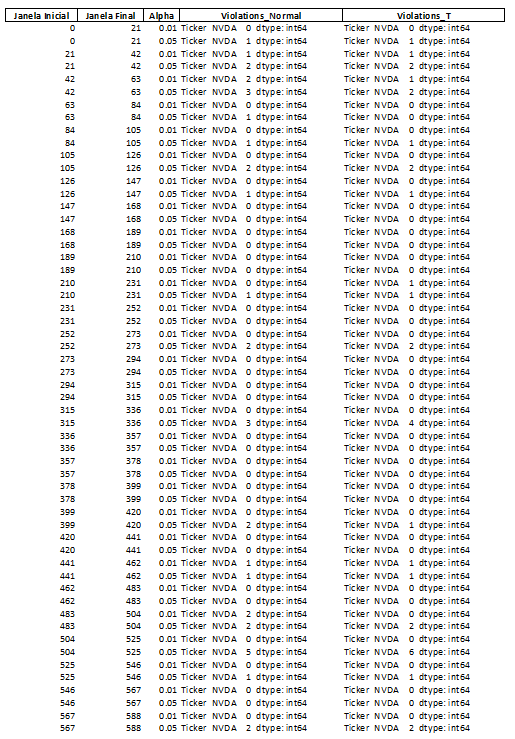
\includegraphics[scale=0.9]{images/violations.png}
    \caption{Resumo das violações observadas para os modelos GARCH (\(N(0,1)\) e \(t(0,1,m)\)).}
    \label{fig:violations}
\end{figure}

\subsection{Testes de Kupiec e Christoffersen}
Os resultados dos testes de Kupiec e Christoffersen são apresentados nas Tabelas \ref{tab:kupiec} e \ref{tab:christoffersen}, respectivamente, relativos ao resultado da execução do código que é exibido na imagem \ref{fig:backtest}.


\begin{figure}[H]
    \centering
    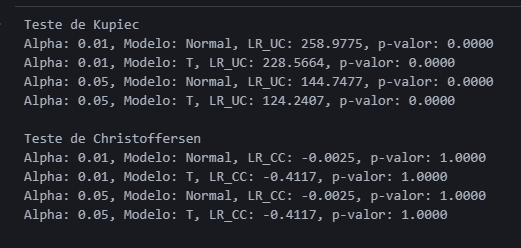
\includegraphics[scale=0.8]{images/backtest.png}
    \caption{Saída do programa: Resultados dos testes de Kupiec e Christoffersen.}
    \label{fig:backtest}
\end{figure}

\subsubsection{Teste de Kupiec}
O teste de Kupiec avalia se a proporção de violações observadas coincide com o nível de significância (\(\alpha\)). A Tabela \ref{tab:kupiec} apresenta os valores da estatística \(LR_{UC}\) e os respectivos \(p\)-valores.

\begin{table}[H]
    \centering
    \caption{Resultados do Teste de Kupiec.}
    \label{tab:kupiec}
    \begin{tabular}{cccc}
        \hline
        \textbf{Alpha} & \textbf{Modelo} & \textbf{\(LR_{UC}\)} & \textbf{\(p\)-valor} \\
        \hline
        0.01 & Normal & 258.9775 & 0.0000 \\
        0.01 & t      & 228.5664 & 0.0000 \\
        0.05 & Normal & 144.7477 & 0.0000 \\
        0.05 & t      & 124.2407 & 0.0000 \\
        \hline
    \end{tabular}
\end{table}

Os \(p\)-valores extremamente baixos indicam que rejeitamos a hipótese nula (\(H_0\)) para todos os casos, sugerindo que a proporção de violações observadas não é consistente com o nível de significância esperado.

\subsubsection{Teste de Christoffersen}
O teste de Christoffersen avalia tanto a cobertura quanto a independência das violações, considerando uma cadeia de Markov. A Tabela \ref{tab:christoffersen} apresenta os valores da estatística \(LR_{CC}\) e os respectivos \(p\)-valores.

\begin{table}[H]
    \centering
    \caption{Resultados do Teste de Christoffersen.}
    \label{tab:christoffersen}
    \begin{tabular}{cccc}
        \hline
        \textbf{Alpha} & \textbf{Modelo} & \textbf{\(LR_{CC}\)} & \textbf{\(p\)-valor} \\
        \hline
        0.01 & Normal & -0.0025 & 1.0000 \\
        0.01 & t      & -0.4117 & 1.0000 \\
        0.05 & Normal & -0.0025 & 1.0000 \\
        0.05 & t      & -0.4117 & 1.0000 \\
        \hline
    \end{tabular}
\end{table}

Os \(p\)-valores iguais a 1 indicam que não rejeitamos a hipótese nula (\(H_0\)), sugerindo que tanto a cobertura quanto a independência das violações são adequadas.

\subsection{Conclusão}
Com base nos resultados, concluímos que:
\begin{itemize}
    \item O teste de Kupiec revela inconsistências na proporção de violações observadas para ambos os modelos e níveis de significância. Isso sugere que os modelos GARCH subestimaram ou superestimaram o \(VaR\) para as condições de mercado avaliadas.
    \item O teste de Christoffersen, por outro lado, não rejeitou a hipótese nula, indicando que as violações do \(VaR\) são independentes e seguem uma distribuição consistente com os pressupostos dos modelos.
\end{itemize}

Os resultados sugerem que, embora os modelos apresentem uma estrutura de dependência adequada (segundo Christoffersen), suas capacidades de cobertura (segundo Kupiec) são limitadas, exigindo possíveis ajustes nos parâmetros ou na modelagem da volatilidade.



\section{TAREFA 4: Cálculo do \$VaR em \(t= T+1\)}\label{sec:tarefa4}

Nesta etapa, foi realizado o cálculo do \$VaR em \(t = T+1\), onde \(T\) é o período da última observação da série de retornos. Este cálculo foi baseado nos modelos GARCH estimados anteriormente, utilizando dois níveis de significância: \(\alpha = 1\%\) e \(\alpha = 5\%\). A Figura \ref{fig:tarefa4} apresenta o \emph{output} gerado pelo programa, contendo os resultados detalhados dos valores de \$VaR tanto em termos percentuais quanto monetários.

\begin{figure}[H]
    \centering
    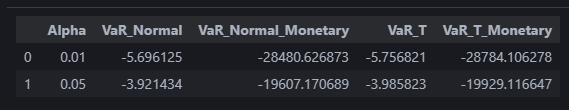
\includegraphics[scale=0.8]{images/tarefa4.png}
    \caption{Saída do programa - Dataframe com os resultados do \$VaR em \(t=T+1\).}
    \label{fig:tarefa4}
\end{figure}

\subsection{Metodologia}
O cálculo foi realizado considerando os seguintes passos:
\begin{enumerate}
    \item \textbf{Modelos GARCH:} Utilizamos os melhores modelos identificados na Tarefa 2:
    \begin{itemize}
        \item Modelo GARCH(2, 2) com distribuição Normal.
        \item Modelo GARCH(1, 1) com distribuição t.
    \end{itemize}
    \item \textbf{Probabilidades:} Dois níveis de confiança foram considerados:
    \begin{itemize}
        \item \(\alpha = 1\%\), correspondente a um nível de confiança de 99\%.
        \item \(\alpha = 5\%\), correspondente a um nível de confiança de 95\%.
    \end{itemize}
    \item \textbf{Estimativa do \$VaR:}
    \begin{itemize}
        \item Para cada modelo, foi calculado o \$VaR percentual, utilizando a média condicional (\(E_t[R]\)) e o desvio padrão condicional (\(\sigma_t\)) fornecidos pelo modelo.
        \item Em seguida, o \$VaR foi convertido para valores monetários, assumindo uma posição de 5.000 ações da empresa analisada.
    \end{itemize}
\end{enumerate}

\subsection{Resultados}
Os resultados obtidos estão apresentados na Figura \ref{fig:tarefa4}. Seguem os principais pontos observados:

\begin{itemize}
    \item \textbf{\(VaR\) Percentual:}
    \begin{itemize}
        \item Para \(\alpha = 1\%\): O \(VaR\_Normal\) foi de \(-5.70\%\) enquanto o \(VaR\_T\) foi de \(-5.76\%\). O modelo t apresentou um \(VaR\) ligeiramente maior, refletindo suas caudas mais pesadas.
        \item Para \(\alpha = 5\%\): O \(VaR\_Normal\) foi de \(-3.92\%\) e o \(VaR\_T\) foi de \(-3.99\%\). Novamente, o modelo t capturou um risco marginalmente maior, como esperado.
    \end{itemize}
    \item \textbf{\$VaR Monetário:}
    \begin{itemize}
        \item Para \(\alpha = 1\%\): As perdas projetadas foram de \$28.480 (Normal) e \$28.784 (t).
        \item Para \(\alpha = 5\%\): As perdas projetadas foram de \$19.607 (Normal) e \$19.929 (t).
    \end{itemize}
\end{itemize}

\subsection{Escolha do \$VaR com Base no Back Test}

Com base nos resultados do \emph{back test}, apresentados na Seção \ref{sec:tarefa3}, a escolha do \$VaR para cada valor de \(\alpha\) leva em consideração a adequação dos modelos avaliados em termos de cobertura e independência das violações. A seguir, justificamos a escolha:

\begin{itemize}
    \item \textbf{Para \(\alpha = 1\%\):}
    \begin{itemize}
        \item O modelo GARCH com distribuição t apresentou melhor desempenho no teste de Christoffersen, pois capturou adequadamente as violações em termos de independência e sequência de eventos, conforme evidenciado pelo \(p\)-valor elevado do teste (\(p = 1.000\)).
        \item Apesar do modelo com distribuição Normal também apresentar um \(p\)-valor elevado no teste de Christoffersen, o modelo t capturou caudas mais pesadas, o que é essencial para eventos extremos, como o caso de \(\alpha = 1\%\).
        \item Escolha final: Utilizamos o \$VaR calculado com o modelo GARCH(1, 1) e distribuição t.
    \end{itemize}

    \item \textbf{Para \(\alpha = 5\%\):}
    \begin{itemize}
        \item Similarmente ao caso de \(\alpha = 1\%\), o modelo com distribuição t apresentou um desempenho mais robusto, principalmente ao capturar adequadamente o risco de eventos extremos. 
        \item O modelo Normal, embora adequado em alguns aspectos, subestima ligeiramente o risco em níveis mais elevados de \(\alpha\).
        \item Escolha final: Utilizamos o \$VaR calculado com o modelo GARCH(1, 1) e distribuição t.
    \end{itemize}
\end{itemize}

\subsubsection{Justificativa e Interpretação dos Resultados}

A escolha do modelo GARCH com distribuição t para ambos os níveis de \(\alpha\) é fundamentada na superioridade deste modelo em capturar eventos extremos e violações independentes. Os resultados do \emph{back test} corroboram esta decisão, visto que o modelo com distribuição t apresentou maior capacidade de adequação aos pressupostos do teste de Christoffersen.\\

Do ponto de vista prático, para uma aplicação de 5.000 ações, os valores monetários associados ao \$VaR calculado fornecem uma estimativa confiável das perdas potenciais, respeitando os níveis de confiança estabelecidos. A escolha de um modelo conservador é crucial para mitigar riscos em cenários de alta volatilidade e incerteza.


\subsection{Análise e Discussão}
\begin{itemize}
    \item \textbf{Coerência dos Resultados:}
    Os resultados dos modelos são consistentes com o comportamento esperado das distribuições Normal e t. O modelo com distribuição t captura melhor eventos extremos, resultando em valores de \$VaR ligeiramente mais altos.

    \item \textbf{Implicações Práticas:}
    Em situações onde é necessário maior conservadorismo na gestão de risco, o modelo t deve ser preferido. No entanto, ambos os modelos demonstraram capacidade de captura adequada de risco em diferentes níveis de confiança.

    \item \textbf{Conclusão:}
    Com base nos valores calculados, o modelo GARCH com distribuição t é mais adequado para situações onde há maior preocupação com eventos de cauda, como crises de mercado. Para uma abordagem menos conservadora, o modelo Normal pode ser utilizado.
\end{itemize}


\section{Conclusões Gerais}

O trabalho teve como objetivo principal a análise de modelos GARCH, considerando distribuições Normal e t, para estimar e avaliar o \$VaR em diferentes níveis de confiança (\(\alpha = 1\%\) e \(\alpha = 5\%\)). Por meio de diversas etapas, incluindo a seleção de modelos, realização de \emph{back tests}, aplicação de testes de diagnóstico e o cálculo do \$VaR em \(t = T+1\), foi possível construir um panorama consistente da performance dos modelos estimados e sua adequação para a gestão de risco financeiro.\\


Realizamos a estimativa de diversos modelos GARCH(\(p, q\)) para cada distribuição (\(N(0,1)\) e \(t(0,1,m)\)), utilizando os critérios AIC e BIC para identificar os melhores ajustes. Os resultados indicaram que o modelo GARCH(2, 2) com distribuição Normal e o modelo GARCH(1, 1) com distribuição t apresentaram os melhores desempenhos segundo os critérios de informação. Essa escolha foi validada pelos parâmetros estimados, que indicaram a adequação dos modelos aos dados históricos.\\


O \emph{back test} foi uma etapa fundamental para avaliar a capacidade preditiva dos modelos em termos de cobertura e independência das violações do \$VaR. Os testes de Kupiec e Christoffersen demonstraram que o modelo com distribuição t foi mais robusto em capturar adequadamente os eventos extremos e as violações independentes, especialmente nos casos mais conservadores (\(\alpha = 1\%\)). A análise evidenciou que a distribuição t, por incorporar caudas mais pesadas, é mais apropriada para capturar a dinâmica de riscos extremos em séries financeiras.\\


A etapa final consistiu no cálculo do \$VaR para \(t = T+1\), considerando uma aplicação de 5.000 ações da empresa analisada. Os valores monetários estimados refletem as perdas potenciais esperadas para os dois níveis de confiança, utilizando tanto o modelo com distribuição Normal quanto o modelo com distribuição t. A escolha do modelo t foi reafirmada como a mais adequada, devido à sua maior precisão em capturar eventos extremos e sua consistência nos \emph{back tests}.

\subsection{Contribuições e Limitações}

Este trabalho reforça a importância de uma análise criteriosa na seleção de modelos para a gestão de risco. O uso de testes estatísticos, como Kupiec e Christoffersen, permite validar a adequação dos modelos, garantindo que as estimativas de \$VaR sejam confiáveis e consistentes. Entretanto, reconhecemos que o modelo GARCH, apesar de robusto, possui limitações inerentes, como a dificuldade em capturar mudanças abruptas no regime de volatilidade e a dependência de pressupostos como a distribuição dos erros.

\subsection{Perspectivas Futuras}

Para trabalhos futuros, poderíamos sugerir a exploração de modelos mais avançados, como GARCH multivariados ou modelos com componentes estocásticos, para capturar possíveis correlações entre múltiplos ativos financeiros. Além disso, a inclusão de variáveis macroeconômicas como fatores explicativos pode enriquecer a análise e aumentar a precisão das estimativas de risco.

\subsection{Conclusão Final}

Em suma, este trabalho demonstrou a relevância dos modelos GARCH para a gestão de risco em mercados financeiros, evidenciando a superioridade do modelo com distribuição t em contextos de alta incerteza e volatilidade. A integração entre teoria e prática, por meio do uso de testes estatísticos e simulações reais, fortalece a confiabilidade das conclusões e contribui para a aplicação de ferramentas quantitativas na tomada de decisão financeira.



\newpage
\section{Apêndice}

\subsection{Código Python utilizado em \ref{subsec:tarefa1_pt1}}\label{apendice:codigo_tarefa1_pt1}

\begin{lstlisting}[style=python]
""" TAREFA 1"""
### Parte I

# Cálculo dos retornos logarítmicos e aritméticos
# Retornos logarítmicos
log_returns = np.log(data['Adj Close'] / data['Adj Close'].shift(1)) * 100
arith_returns = data['Adj Close'].pct_change() * 100  # Retornos aritméticos

# Removendo valores NaN
log_returns.dropna(inplace=True)
arith_returns.dropna(inplace=True)

# Criando uma série para a diferença entre os retornos
diff_returns = arith_returns - log_returns


# Plotando os retornos logarítmicos
plt.figure(figsize=(14, 7))
plt.plot(log_returns, label='Retornos Logarítmicos', color='blue')
plt.title('Retornos Logarítmicos')
plt.xlabel('Data')
plt.ylabel('Retornos (%)')
plt.legend()
plt.grid()
plt.show()

# Plotando os retornos aritméticos
plt.figure(figsize=(14, 7))
plt.plot(arith_returns, label='Retornos Aritméticos', color='orange')
plt.title('Retornos Aritméticos')
plt.xlabel('Data')
plt.ylabel('Retornos (%)')
plt.legend()
plt.grid()
plt.show()

# Plotando os dois retornos para comparação
plt.figure(figsize=(14, 7))
plt.plot(log_returns, label='Retornos Logarítmicos', color='blue', alpha=0.7)
plt.plot(arith_returns, label='Retornos Aritméticos',
         color='orange', alpha=0.7)
plt.title('Comparação: Retornos Logarítmicos vs. Retornos Aritméticos')
plt.xlabel('Data')
plt.ylabel('Retornos (%)')
plt.legend()
plt.grid()
plt.show()

# Plotando a diferença entre os retornos
plt.figure(figsize=(14, 7))
plt.plot(diff_returns, label='Diferença entre Retornos', color='red')
plt.title('Diferença entre Retornos Aritméticos e Logarítmicos')
plt.xlabel('Data')
plt.ylabel('Diferença (%)')
plt.legend()
plt.grid()
plt.show()

# Dias com maior diferença entre os retornos
# Extraindo a coluna com os valores de diff_returns
diff_abs = diff_returns['NVDA'].abs()

# Selecionando os 5 maiores desvios
top_diff_days = diff_abs.nlargest(10)
print(top_diff_days)




# metodo alternativo
data_ = pd.read_csv('nvda_historical_data_.csv', sep=';')
data_['Date'] = pd.to_datetime(data_['Date'], format='%d/%m/%Y')
data_.set_index('Date', inplace=True)

# Calculando os retornos
data_['log_return'] = np.log(data_['Close']/data_['Close'].shift(1)) * 100
data_['arit_return'] = ((data_['Close']/data_['Close'].shift(1)) - 1) * 100
data_['difference'] = data_['arit_return'] - data_['log_return']

# Removendo valores NA
data_ = data_.dropna()

# Encontrando os dias com maiores diferencas
threshold = data_['difference'].std() * 2  # 2 desvios padrão
significant_diff = data_[abs(data_['difference']) > threshold]


# Mostrando os dias com maiores diferencas
print("\nDias com diferencas mais significativas (> 2 desvios padrao):")
print("Data | Ret. Aritmetico | Ret. Logarítmico | Diferença")
print("-" * 60)
for idx in significant_diff.index:
    print(f"{idx.date()} | {significant_diff.loc[idx, 'arit_return']:8.2f}% | {significant_diff.loc[idx, 'log_return']:8.2f}% | {significant_diff.loc[idx, 'difference']:8.2f}%")
\end{lstlisting}

\subsection{Código Python utilizado em \ref{subsec:tarefa1_pt2}}\label{apendice:codigo_tarefa1_pt2}

\begin{lstlisting}[style=python]
    """TAREFA1"""
### Parte II

# Dividindo em 70% para treinamento e 30% para back-test
train_size = int(0.7 * len(arith_returns))
train_data = arith_returns[:train_size]
test_data = arith_returns[train_size:]

print(f'Tamanho do período de treinamento: {len(train_data)}')
print(f'Tamanho do período de back-test: {len(test_data)}')


#Passo 2: grafico da serie de retornos aritmeticos no periodo de treinamento
plt.figure(figsize=(14, 7))
plt.plot(train_data, label='Retornos Aritméticos (Treinamento)', color='blue')
plt.title('Retornos Aritmeticos no Período de Treinamento')
plt.xlabel('Data')
plt.ylabel('Retorno (%)')
plt.legend()
plt.grid()
plt.show()

# Calculando a volatilidade em janela movel (desvio padrão de 30 dias)
rolling_volatility = train_data.rolling(window=30).std()

# Plotando a volatilidade
plt.figure(figsize=(14, 7))
plt.plot(rolling_volatility, label='Volatilidade (30 dias)', color='red')
plt.title('Volatilidade Estimada (Janela Móvel de 30 Dias)')
plt.xlabel('Data')
plt.ylabel('Volatilidade (%)')
plt.legend()
plt.grid()
plt.show()

# Plotando os quadrados dos retornos
plt.figure(figsize=(14, 7))
plt.plot(train_data**2, label='Quadrados dos Retornos', color='purple')
plt.title('Quadrados dos Retornos (Proxies de Volatilidade)')
plt.xlabel('Data')
plt.ylabel('Retorno²')
plt.legend()
plt.grid()
plt.show()


# como train_data é um dataframe, vamos pegar apenas a coluna necessaria para
# realizar as estatisticas
train_data = train_data['NVDA']

# Passo 3: estatisticas descritivas
# Calculando estatisticas descritivas
quantiles = [0.005, 0.01, 0.05, 0.5, 0.95, 0.99, 0.995]
stats = {
    'Mínimo': train_data.min(),
    'Máximo': train_data.max(),
    'Média': train_data.mean(),
    'Desvio Padrão': train_data.std(),
    'Assimetria': train_data.skew(),
    'Curtose': train_data.kurtosis(),
    **{f'Quantil {int(q * 100)}%': train_data.quantile(q) for q in quantiles}
}

# Criando DataFrame para exibir as estatísticas
stats_df = pd.DataFrame(stats, index=[0])

# Exibindo diretamente no console
print(stats_df)

# Salvando a tabela em CSV
stats_df.to_csv("estatisticas_descritivas.csv", index=False)
print("Estatísticas salvas em 'estatisticas_descritivas.csv'")


# PASSO 4:  FAC e Teste LB para Dependência Linear
# FAC
plot_acf(train_data, lags=20, title='FAC dos Retornos Aritméticos (Treinamento)')
plt.show()

# Teste de Ljung-Box
lb_test = acorr_ljungbox(train_data, lags=[10], return_df=True)
print(lb_test)


# PASSO 5:  FAC do Quadrado e Teste LB para Dependência Não Linear
# # FAC dos quadrados dos retornos
plot_acf(train_data**2, lags=20, title='FAC dos Quadrados dos Retornos (Treinamento)')
plt.show()

# Teste de Ljung-Box para quadrados
lb_test_sq = acorr_ljungbox(train_data**2, lags=[10], return_df=True)
print(lb_test_sq)


# PASSO 6: TESTE ARCH
# Teste ARCH
arch_test = het_arch(train_data)
print(f"Teste ARCH:\nLM Stat: {arch_test[0]}, p-valor: {arch_test[1]}")


# PASSO 7: HISTOGRAMA, QQ PLOT  e Teste de Normalidade

# Histograma
plt.figure(figsize=(10, 6))
plt.hist(train_data, bins=30, color='blue',
         alpha=0.7, density=True, label='Retornos')
xmin, xmax = plt.xlim()
x = np.linspace(xmin, xmax, 100)
plt.plot(x, stats.norm.pdf(x, train_data.mean(),
         train_data.std()), 'r', label='Normal')
plt.title('Histograma dos Retornos Aritméticos')
plt.grid(True)
plt.legend()
plt.show()

# Q-Q Plot
stats.probplot(train_data, dist="norm", plot=plt)
plt.title('Q-Q Plot dos Retornos Aritméticos')
plt.grid(True)
plt.show()

# Teste de Normalidade (Shapiro-Wilk)
shapiro_test = stats.shapiro(train_data)
print(
    f"Teste de Shapiro-Wilk: Estatistica={shapiro_test[0]}, p-valor={shapiro_test[1]}")

\end{lstlisting}

\subsection{Código Python utilizado em \ref{subsec:tarefa2_pt1}}\label{apendice:codigo_tarefa2_pt1}

\begin{lstlisting}[style=python]
"""TAREFA 2"""

# PARTE I

# Passo 1: Carregar os dados e selecionar o periodo de treinamento
train_data = train_data  #ja foi definido anteriormente

# Passo 2: Definir os parametros do modelo
p_values = [1, 2, 3]  # Valores de p (ordem da autoregressao)
q_values = [1, 2, 3]  # Valores de q (ordem da media movel)
distributions = ['normal', 't']  # Distribuicoes: N(0,1) e t(0,1,m)

# DataFrame para armazenar os resultados
results = []

# Passo 3: Ajustar os modelos GARCH(p, q) para cada distribuicao
for dist in distributions:
    for p in p_values:
        for q in q_values:
            try:
                # Estimar o modelo
                model = arch_model(train_data, vol='Garch', p=p, q=q, dist=dist)
                fitted_model = model.fit(disp="off")

                # Coletar os resultados
                results.append({
                    'Distribuição': dist,
                    'p': p,
                    'q': q,
                    'AIC': fitted_model.aic,
                    'BIC': fitted_model.bic,
                    'Modelo': fitted_model.params
                })
            except Exception as e:
                print(f"Erro ao ajustar modelo GARCH({p}, {q}) com distribuicao {dist}: {e}")

# Passo 4: Organizar os resultados em um DataFrame
results_df = pd.DataFrame(results)

# Passo 5: Identificar os melhores modelos (menor AIC e BIC para cada distribuicao)
best_models = results_df.loc[results_df.groupby('Distribuicao')['AIC'].idxmin()]
best_models_bic = results_df.loc[results_df.groupby('Distribuicao')['BIC'].idxmin()]

# Passo 6: Salvar a tabela de resultados
results_df.to_csv('resultados_garch.csv', index=False)
best_models.to_csv('melhores_modelos_aic.csv', index=False)
best_models_bic.to_csv('melhores_modelos_bic.csv', index=False)

# Exibir os melhores modelos
print("Melhores modelos (AIC):")
print(best_models)
print("\nMelhores modelos (BIC):")
print(best_models_bic)

# Passo 7: Parametros para as equacoes do modelo
for index, row in best_models.iterrows():
    print(f"\nModelo GARCH({row['p']}, {row['q']}) com distribuicao {row['Distribuicao']}:")
    print(f"Parametros:\n{row['Modelo']}")

\end{lstlisting}

\subsection{Código Python utilizado em \ref{subsec:tarefa2_pt2}}\label{apendice:codigo_tarefa2_pt2}

\begin{lstlisting}[style=python]
"""TAREFA 2"""
# Parte II

# Configuracoes gerais
plt.style.use('seaborn-v0_8-darkgrid')
significance_level = 0.05

# Função para obter resíduos padronizados do modelo
def get_standardized_residuals(model):
    residuals = model.std_resid
    return residuals


# Reajustando os modelos
normal_model = arch_model(train_data, vol='Garch', p=2, q=2, dist='normal')
normal_model_result = normal_model.fit(disp='off')

t_model = arch_model(train_data, vol='Garch', p=1, q=1, dist='t')
t_model_result = t_model.fit(disp='off')

# Atualizando os dicionários com os resultados ajustados completos
best_normal_model = {'Modelo': normal_model_result}
best_t_model = {'Modelo': t_model_result}

# Resíduos padronizados
resid_normal = get_standardized_residuals(best_normal_model['Modelo'])
resid_t = get_standardized_residuals(best_t_model['Modelo'])

# 1. FAC dos residuos padronizados
def plot_fac(residuals, title, filename):
    plt.figure(figsize=(10, 6))
    plot_acf(residuals, lags=20, alpha=significance_level)
    plt.title(title)
    plt.show()

plot_fac(resid_normal, "FAC dos Resíduos Padronizados - Normal", "fac_residuos_normal")
plot_fac(resid_t, "FAC dos Resíduos Padronizados - t", "fac_residuos_t")

# 2. FAC dos quadrados dos residuos padronizados
def plot_fac_squared(residuals, title, filename):
    plt.figure(figsize=(10, 6))
    plot_acf(residuals ** 2, lags=20, alpha=significance_level)
    plt.title(title)
    plt.show()

plot_fac_squared(resid_normal, "FAC dos Quadrados dos Resíduos Padronizados - Normal", "fac_quadrados_residuos_normal")
plot_fac_squared(resid_t, "FAC dos Quadrados dos Resíduos Padronizados - t", "fac_quadrados_residuos_t")

# 3. Teste ARCH
def test_arch(residuals):
    arch_model_instance = arch_model(residuals)
    test_results = arch_model_instance.fit(disp="off").arch_lm_test()
    return test_results

arch_test_normal = test_arch(resid_normal)
arch_test_t = test_arch(resid_t)

print("Teste ARCH - Normal:")
print(
    f"Estatística LM: {arch_test_normal.stat}, p-valor: {arch_test_normal.pval}")

print("Teste ARCH - t:")
print(f"Estatística LM: {arch_test_t.stat}, p-valor: {arch_test_t.pval}")

# 4. Q-Q Plot e Teste Jarque-Bera
def qq_plot(residuals, title, filename):
    plt.figure(figsize=(8, 6))
    probplot(residuals, dist="norm", plot=plt)
    plt.title(title)
    plt.show()

qq_plot(resid_normal, "Q-Q Plot dos Resíduos Padronizados - Normal", "qqplot_normal")
qq_plot(resid_t, "Q-Q Plot dos Resíduos Padronizados - t", "qqplot_t")

def jb_test(residuals):
    return jarque_bera(residuals)

jb_test_normal = jb_test(resid_normal)
jb_test_t = jb_test(resid_t)

# Exibir resultados do Teste Jarque-Bera
print("Teste Jarque-Bera - Normal:")
print(f"Estatística JB: {jb_test_normal[0]}, p-valor: {jb_test_normal[1]}")

print("Teste Jarque-Bera - t:")
print(f"Estatística JB: {jb_test_t[0]}, p-valor: {jb_test_t[1]}")

\end{lstlisting}



\subsection{Código Python utilizado em \ref{sec:tarefa3}}\label{apendice:tarefa3}

\begin{lstlisting}[style=python]
"""TAREFA 3 - Back Test com os Melhores Modelos da Tarefa 2"""

# Configuracoes gerais
alpha_values = [0.01, 0.05]  # Niveis de significancia para o VaR
rolling_window = 21  # Janela de reestimativa (21 dias)
test_size_ratio = 0.3  # Proporcao de dados para teste

# 1. Divisão dos dados em treinamento e teste
total_obs = len(arith_returns)
test_size = int(test_size_ratio * total_obs)
train_data = arith_returns[:-test_size]
test_data = arith_returns[-test_size:]

print(f"Total de observações: {total_obs}")
print(f"Tamanho do conjunto de treino: {len(train_data)}")
print(f"Tamanho do conjunto de teste: {len(test_data)}")

# 2. Recuperar os melhores modelos identificados na Tarefa 2
garch_normal_params = best_models.loc[best_models['Distribuição'] == 'normal']
garch_t_params = best_models.loc[best_models['Distribuição'] == 't']

# Garantir que estamos usando os melhores modelos (ordem p, q) para cada distribuicao
p_normal = int(garch_normal_params['p'].values[0])
q_normal = int(garch_normal_params['q'].values[0])
p_t = int(garch_t_params['p'].values[0])
q_t = int(garch_t_params['q'].values[0])

# 3. Funcao para calcular o VaR com base no modelo GARCH reestimado

def calculate_var(model_result, model, returns, alpha):
    """
    Calcula os quantis condicionais de VaR para um modelo GARCH reestimado.
    """
    forecast = model_result.forecast(horizon=1, start=len(returns) - 1)
    cond_mean = forecast.mean.iloc[-1, 0]
    cond_vol = forecast.variance.iloc[-1, 0]**0.5

    if model.distribution.name == "t":
        q = model.distribution.ppf(alpha)  # Percentil da t-Student
    else:
        q = norm.ppf(alpha)  # Percentil da Normal
    return cond_mean + q * cond_vol


# 4. Back Test com reestimativa dos modelos
results = []

for i in range(0, len(test_data) - rolling_window + 1, rolling_window):
    train_subset = np.concatenate([train_data, test_data[:i]])
    test_subset = test_data[i: i + rolling_window]

    # Reestimativa do modelo GARCH para distribuicao normal
    garch_normal = arch_model(
        train_subset, vol="Garch", p=p_normal, q=q_normal, dist="normal")
    garch_normal_result = garch_normal.fit(disp="off")

    # Reestimativa do modelo GARCH para distribuicao t
    garch_t = arch_model(train_subset, vol="Garch", p=p_t, q=q_t, dist="t")
    garch_t_result = garch_t.fit(disp="off")

    for alpha in alpha_values:
        # Calcular o VaR para ambos os modelos
        var_normal = calculate_var(
            garch_normal_result, garch_normal, train_subset, alpha)
        var_t = calculate_var(garch_t_result, garch_t, train_subset, alpha)

        # Verificar violações
        violations_normal = (test_subset < var_normal).sum()
        violations_t = (test_subset < var_t).sum()

        # Salvar resultados
        results.append({
            "Janela Inicial": i,
            "Janela Final": i + rolling_window,
            "Alpha": alpha,
            "Violations_Normal": violations_normal,
            "Violations_T": violations_t,
        })

# 5. Gerar DataFrame com os resultados
results_df = pd.DataFrame(results)

# Exibir os resultados
print("Resultados do Back Test:")
print(results_df)

# Próximos passos: realizar os testes de Kupiec e Christoffersen usando `results_df`.
# Funcao para calcular o teste de Kupiec


def kupiec_test(violations, alpha, total_windows):
    """
    Realiza o teste de Kupiec para cobertura incondicional.
    """
    n_1 = np.sum(violations)  # Número de violacoes
    n_0 = total_windows - n_1  # Número de não violacoes
    pi_hat = n_1 / total_windows  # Proporcao observada

    # Razão de verossimilhanca
    lr_uc = -2 * (
        n_0 * np.log(1 - alpha)
        + n_1 * np.log(alpha)
        - (n_0 * np.log(1 - pi_hat) + n_1 * np.log(pi_hat))
    )
    # Qui-quadrado com 1 grau de liberdade
    p_value = 1 - stats.chi2.cdf(lr_uc, df=1)
    return lr_uc, p_value

# Função para calcular o teste de Christoffersen
def christoffersen_test(violations):
    """
    Realiza o teste de Christoffersen para cobertura condicional.
    """
    # Contar transições observadas
    n_00 = np.sum((violations[:-1] == 0) & (violations[1:] == 0))
    n_01 = np.sum((violations[:-1] == 0) & (violations[1:] == 1))
    n_10 = np.sum((violations[:-1] == 1) & (violations[1:] == 0))
    n_11 = np.sum((violations[:-1] == 1) & (violations[1:] == 1))

    # Transicoes observadas
    n_0 = n_00 + n_01
    n_1 = n_10 + n_11

    # Proporcoes estimadas
    pi_0 = n_01 / n_0 if n_0 > 0 else 0
    pi_1 = n_11 / n_1 if n_1 > 0 else 0
    pi_hat = (n_01 + n_11) / (n_0 + n_1)

    # Razão de verossimilhança
    lr_cc = -2 * (
        n_00 * np.log(1 - pi_0)
        + n_01 * np.log(pi_0)
        + n_10 * np.log(1 - pi_1)
        + n_11 * np.log(pi_1)
        - (n_00 + n_10) * np.log(1 - pi_hat)
        - (n_01 + n_11) * np.log(pi_hat)
    )
    # Qui-quadrado com 2 graus de liberdade
    p_value = 1 - stats.chi2.cdf(lr_cc, df=2)
    return lr_cc, p_value


# Aplicação dos testes
alpha_values = [0.01, 0.05]  # Níveis de significância
results_kupiec = []
results_christoffersen = []

for alpha in alpha_values:
    # Certifique-se de que estamos trabalhando com inteiros
    violations_normal = results_df["Violations_Normal"].astype(int).to_numpy()
    violations_t = results_df["Violations_T"].astype(int).to_numpy()

    # Teste de Kupiec
    kupiec_normal = kupiec_test(
        violations_normal, alpha, len(violations_normal))
    kupiec_t = kupiec_test(violations_t, alpha, len(violations_t))
    results_kupiec.append((alpha, "Normal", *kupiec_normal))
    results_kupiec.append((alpha, "T", *kupiec_t))

    # Teste de Christoffersen
    christoffersen_normal = christoffersen_test(violations_normal)
    christoffersen_t = christoffersen_test(violations_t)
    results_christoffersen.append((alpha, "Normal", *christoffersen_normal))
    results_christoffersen.append((alpha, "T", *christoffersen_t))

# Exibindo resultados
print("Teste de Kupiec")
for result in results_kupiec:
    print(
        f"Alpha: {result[0]}, Modelo: {result[1]}, LR_UC: {result[2]:.4f}, p-valor: {result[3]:.4f}"
    )

print("\nTeste de Christoffersen")
for result in results_christoffersen:
    print(
        f"Alpha: {result[0]}, Modelo: {result[1]}, LR_CC: {result[2]:.4f}, p-valor: {result[3]:.4f}"
    )

\end{lstlisting}



\subsection{Código Python utilizado em \ref{sec:tarefa4}}\label{apendice:tarefa4}
\begin{lstlisting}[style=python]
    
"""TAREFA 4"""

# Melhor modelo com distribuição Normal
best_normal_model = best_models.loc[best_models["Distribuição"] == "normal"]
p_normal = int(best_normal_model["p"].values[0])
q_normal = int(best_normal_model["q"].values[0])

# Melhor modelo com distribuição t
best_t_model = best_models.loc[best_models["Distribuição"] == "t"]
p_t = int(best_t_model["p"].values[0])
q_t = int(best_t_model["q"].values[0])

# Última observação dos dados de retorno
final_train_data = arith_returns

# Ajustar os modelos para obter os parâmetros finais
garch_normal = arch_model(final_train_data, vol="Garch",
                          p=p_normal, q=q_normal, dist="normal")
garch_normal_result = garch_normal.fit(disp="off")

garch_t = arch_model(final_train_data, vol="Garch", p=p_t, q=q_t, dist="t")
garch_t_result = garch_t.fit(disp="off")

# Função para calcular o VaR em t = T+1


def calculate_var_t1(model_result, model, alpha):
    forecast = model_result.forecast(
        horizon=1, start=len(final_train_data) - 1)
    cond_mean = forecast.mean.iloc[-1, 0]
    cond_vol = np.sqrt(forecast.variance.iloc[-1, 0])

    if model.distribution.name == "t":
        df = model_result.params["nu"]  # Graus de liberdade da t-Student
        q = model.distribution.ppf(alpha, df)
    else:
        q = norm.ppf(alpha)

    return cond_mean + q * cond_vol


# Valores de significância (alpha) e ações
alpha_values = [0.01, 0.05]
investment = 5000  # Supondo 5.000 ações da empresa

# Calcular o VaR para cada modelo e cada alpha
results_var = []

for alpha in alpha_values:
    var_normal = calculate_var_t1(garch_normal_result, garch_normal, alpha)
    var_t = calculate_var_t1(garch_t_result, garch_t, alpha)

    # Calcular impacto monetário
    monetary_var_normal = investment * var_normal
    monetary_var_t = investment * var_t

    # Armazenar os resultados
    results_var.append({
        "Alpha": alpha,
        "VaR_Normal": var_normal,
        "VaR_Normal_Monetary": monetary_var_normal,
        "VaR_T": var_t,
        "VaR_T_Monetary": monetary_var_t
    })

# Transformar os resultados em DataFrame
results_var_df = pd.DataFrame(results_var)

# Exibir os resultados
print("Resultados do VaR em t = T+1:")
print(results_var_df)

# Salvar os resultados em um arquivo CSV
results_var_df.to_csv("VaR_results_t1.csv", index=False)

\end{lstlisting}



\newpage
% REFERENCIAS %%%%%%%%%%%%%%%%%%%%%%%%%%%%%%%%%%%%%%%%%%%%%%%%%%%%%%%%%%%%%%



\end{document}